\documentclass[serif,11pt,aspectratio=1610,table]{beamer}
\usepackage{listings}
\usepackage{verbatim}
\usepackage[utf8x]{inputenc}
\usepackage{default}
\usetheme{Copenhagen}
\usepackage{hyperref}
\usepackage{caption}
\usepackage{beamerthemesplit}
\usepackage{mathtools}  
\usepackage{amsmath}
\usepackage{fancyvrb}
\usepackage{framed,color}
\usepackage{ragged2e}
\usepackage{listings}
\usepackage{multirow}
\usepackage{color, colortbl}
%\usepackage{multicolumn}
\usepackage{xcolor,colortbl}
%\usepackage[T1]{fontenc} %For BG IMAGE
\usepackage{graphicx} %For BG Image
\setbeamersize{text margin left=.5cm,text margin right=.5cm} 
\setbeamertemplate{frametitle}[default][center]
%\setbeamercolor{background canvas}{bg=green!1} Set BG colcor
%%%%%%%BG IMAGE BEGIN
%\usebackgroundtemplate
%{%
%    \includegraphics[width=\paperwidth,height=\paperheight]{1203m.png}%
%}
\usepackage{ccicons}
%%%%%%%%%%%BG IMAGE END
%\usepackage{fontspec}
%\usepackage{qtree}
\definecolor{shadecolor}{HTML}{FF7F00}
%{rgb}{1,0.5,0}
%\logo{
\includegraphics[height=.7cm,width=1cm]{Tux.png}}
%\usepackage{multimedia} %for movie
%\movie[width=3cm,height=2cm,poster,showcontrols=true]{}{sample_movie.avi} % autostart start=10
%\logo{\includegraphics[height=2cm]{bucky.png}} %logo
%\sound[autostart,samplingrate=22050]{}{applause.au}
\title {Elements of Text Mining}
\subtitle {Theory to Practice}
%\subtitle {}
\author[Jaganadh G] {Jaganadh G \\ http://jaganadhg.in \\ \ccbysa}
%\logo{\ccbysa}
\date {}


\begin{document}

\begin{frame}
 \maketitle
\end{frame}

\begin{frame}[fragile]
 \frametitle{Tokenization}
 \begin{block}<+->{Tokenization}
  Tokenization is the process of breaking a stream of text up into words, phrases, symbols, or other meaningful elements called tokens. The list of tokens becomes input for further processing such as parsing or text mining.
 \end{block}

\begin{block}<+->{Tokenizig text with Python}

\footnotesize
\begin{verbatim}
import re

def tokenize(text):
  tokenizer = re.compile('\\W*')
  return tokenizer.split(text.lower())

doc = "John likes to watch movies. Mary likes too"
words = tokenize(doc)
print words
\end{verbatim}
%\end{beamercolorbox}

\end{block}

\end{frame}

\begin{frame}[fragile]
 \frametitle{Twokenization}
\scriptsize
Rise of social media introduced new orthographic patterns in digital text. Typical example is a tweet; where people use abbreviated forms of words emoticons, hash-tags etc.. Generic text tokenization techniques wont yield good result in separating words in social media text, like tweets. A good social media tokenizer has to take care of emoticons, hash-tags, shortened urls etc... \\
Social media tokenization with Python using happyfuntokenizing \footnote{\url{https://bitbucket.org/jaganadhg/twittertokenize}}
\footnotesize
\begin{verbatim}
from happyfuntokenizing import Tokenizer

def twokenize(tweet,pc=True):
    twokenizer = Tokenizer(preserve_case=pc)

    return twokenizer.tokenize(tweet)

tweet = "RT @USER : Relevant 2 clinical text > Recursive neural networks:\
Deep Learning Natural Language Processing #NLProc  http://t.co /"

twokens = tokenize(tweet)
\end{verbatim}

\end{frame}


\begin{frame}[fragile]
 \frametitle{Sentence Tokenization}
\footnotesize
Heuristic sentence boundary detection algorithm \footnote{Chris Manning and Hinrich Schütze, Foundations of Statistical Natural Language Processing, MIT Press. Cambridge, MA: May 1999. }

\footnotesize
\begin{itemize}
 \item Place putative sentence boundaries after all occurrences of  . ? ! ( and maybe ; : -\_)
 \item Move the boundary after following quotation marks, if any.
 \item Disqualify a period boundary in the following circumstances:
    \begin{itemize}
     \item If it is preceded by a known abbreviation of a sort that does not normally occur word finally, but is commonly followed by a capitalized proper name, such as Prof. or vs.
     \item If it is preceded by a known abbreviation and not followed by an uppercase word. This will deal correctly with most usages of abbreviations like etc. or Jr. which can occur sentence medially or finally.
    \end{itemize}
 \item Disqualify a boundary with a ? or ! if:
  \begin{itemize}
   \item It is followed by a lowercase letter (or a known name).
  \end{itemize}
 \item Regard other putative sentence boundaries as sentence boundaries.
\end{itemize}
\end{frame}

\begin{frame}[fragile]
 \frametitle{Sentence Tokenization}

\begin{block}<+->{Sentence Tokenization with Python and NLTK}
\footnotesize
\begin{verbatim}
from nltk.data import load
tokenizer = load('tokenizers/punkt/english.pickle')
text = "How can this be implemented? There are a lot of subtleties, \
such as dot being used in abbreviations."
sents = tokenizer.tokenize(text)
for sent in sents:
  print sent

\end{verbatim}

\end{block}

\end{frame}

\begin{frame}[fragile]
 \frametitle{Counting Words}
\footnotesize
\begin{block}<+->{Word Count - Python}
 \begin{verbatim}

def word_count(text):
  words = tokenize(text)
  word_freq = dict([(word, words.count(word)) for word \
  in set(words)])
  return word_freq

text = "How can this be implemented? There are a lot of \
subtleties, such as dot being used in abbreviations."

wc = word_count(text)

for word,count in wc.items():
  print word , "\t \t", count
 \end{verbatim}

\end{block}

\end{frame}

\begin{frame}[fragile]
 \frametitle{Finding Word Length}
\begin{block}<+->{Word Length}
 \footnotesize
\begin{verbatim}
def word_length(text):
  words = tokenize(text)
  word_length = {}
  [word_length.__setitem__(len(word),1 + \
  word_length.get(len(word),0)) for word in words]
  return word_length

text = "How can this be implemented? There are a lot of \
subtleties, such as dot being used in abbreviations."

wl = word_length(text)

for length, count in wl.items():
  print "There are %d words of length %d " %(count, length)
\end{verbatim}

\end{block}

\end{frame}

\begin{frame}[fragile]
 \frametitle{Word Proportion}
\begin{block}<+->{Word Proportion}
 Let $C$ be a corpus where $(w_{1},w_{2},w_{3},...,w_{n})$ are the words.\\
 $SIZE(C) = length(tokens(C))$ simply total number of words\\
 so $ p(w_{i},C) = \frac{f(w_{i},C)}{SIZE(C)} $ where $f(w_{i},C)$ is the frequency of $w_{i}$ in $C$
\end{block}

\begin{block}<+->{Finding Word Proportion}
 \footnotesize
\begin{verbatim}
from __future__ import division
def word_propo(text):
    words = tokenize(text)
    wc = word_count(text)
    propo = dict([(word, wc[word]/len(words)) for word \
    in set(words)])
    return propo
text = "How can this be implemented? There are a lot of \
        subtleties, such as dot being used in abbreviations."
wp = word_propo(text)
for word, propo in wp.items():
    print word, "\t\t", propo
\end{verbatim}

\end{block}

\end{frame}


\begin{frame}[fragile]
 \frametitle{Words Types and Ratio}
\begin{block}<+>{Words and Types}
 Words and valid tokens from a given corpus $C$ \\
 Types are total distinct tokens in a given corpus $C$ \\
 Example: \\
 $C = $ "I shot an elephant in my pajamas. He saw the fine fat trout in the brook."\\
 There are 16 words and 15 types in $C$. \\
 \footnotesize
 words = ('i', 'shot', 'an', 'elephant', 'in', 'my', 'pajamas', 
 'he', 'saw', 'the', 'fine', 'fat', 'trout', 'in', 'the', 'brook') \\
 types = ('shot', 'i', 'saw', 'elephant', 'brook', 'fine', 'an', 
 'fat', 'in', 'my', 'the', 'he', 'pajamas', 'trout')
\end{block}

\end{frame}

\begin{frame}[fragile]
 \frametitle{Words Types and Ratio}
 \begin{block}<+->{Word Type Ratio}
  $WTR(C) = \frac{WC(C)}{C(T)}$ where $WC(C)$ is total number of words in corpus $C$ and $C(T)$ is the count of types in corpus $C$
 \end{block}
\begin{block}<+->{Finding Word Type Ratio}
 \footnotesize
\begin{verbatim}
def word_type_ratio(text):
    words = tokenize(text)
    ratio = len(words) / len(set(words))
    return ratio

text = "I shot an elephant in my pajamas. He saw the fine \
        fat trout in the brook."
ratio = word_type_ratio(text)
print ratio
\end{verbatim}

\end{block}

\end{frame}

\begin{frame}[fragile]
 \frametitle{Finding top N words}
Python code to find top N words from a text
\footnotesize
\begin{verbatim}
from operator import itemgetter

def top_words(text,n=50):
  wordfreq = word_count(text)
  topwords = sorted(wordfreq.iteritems(), key = itemgetter(1),\
  reverse=True)[:n]
  return topwords

text = open('gpl-2.0.txt','r').read()
topwords = top_words(text,n=50)

for word, count in topwords:
  print "%s \t %d " %(word,count)
\end{verbatim}
\end{frame}

\begin{frame}[fragile]
 \frametitle{Plotting top N words}
Python code to plot top 20 words from a text
\footnotesize
\begin{verbatim}
import numpy as np
import matplotlib.pyplot as plt

def plot_freq(text):
  tfw = top_words(text, n= 20)
  x = range(len(tfw))
  np = len(tfw)
  y = []
  for item in range(np):
    y = y + [tfw[item][1]]

  plt.plot(x,y,'bo',ls='dotted')
  plt.xticks(range(0, len(words) + 1, 1))
  plt.yticks(range(0, max(y) + 1, 10))
  plt.xlabel("Word Ranking")
  plt.ylabel("Word Frequency")
  plt.show()
text = open('gpl-2.0.txt','r').read()
plot_freq(text)
\end{verbatim}

\end{frame}

\begin{frame}
 \frametitle{Top N Words}
\small{Plot of top 50 words from GPL v.2. (without filtering stop words)} \\
%\begin{figure}[h!]
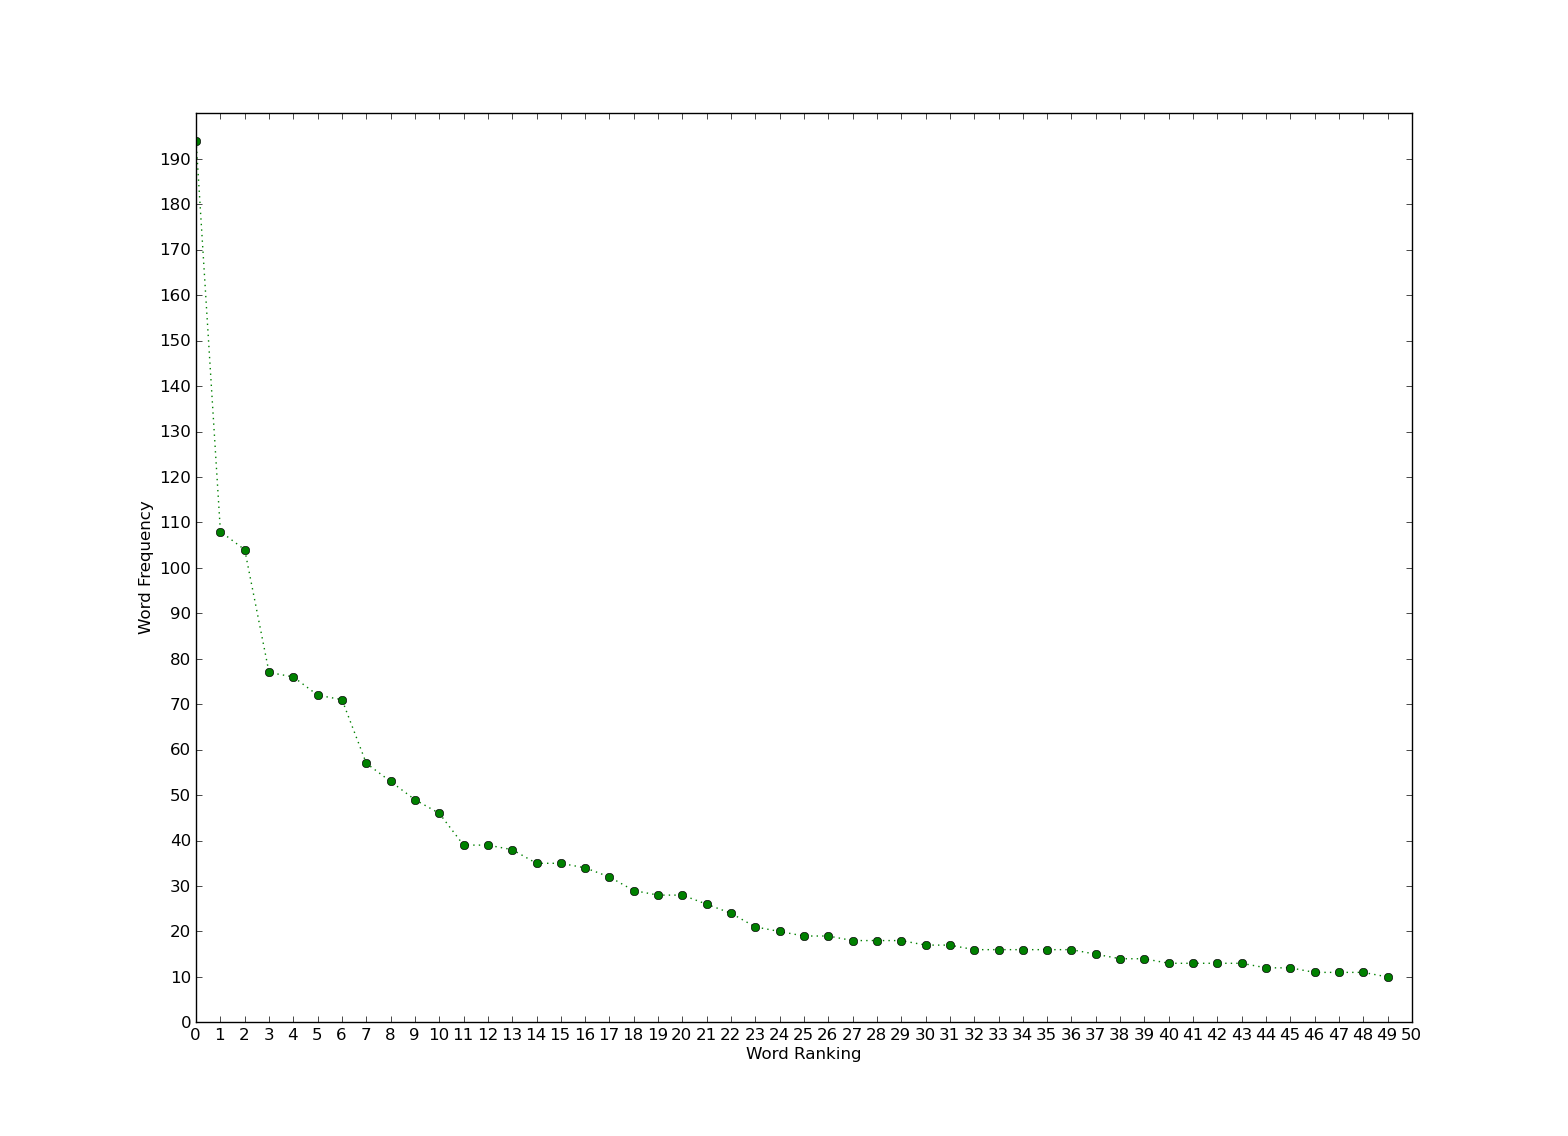
\includegraphics[height=8cm]{freq.png}
% \caption{Plot of top 50 words from GPL v.2. (without filtering stop words)}
%\end{figure}
\end{frame}

\begin{frame}[fragile]
 \frametitle{Plotting top N words}
Python code to plot top 50 words from a text. This plot will show words in the plot.
\tiny
\begin{verbatim}
import numpy as np
import matplotlib.pyplot as plt

def plot_freq_tag(text):
  tfw = top_words(text, n= 50)
  words = [tfw[i][0] for i in range(len(tfw))]
  x = range(len(tfw))
  np = len(tfw)
  y = []
  for item in range(np):
    y = y + [tfw[item][1]]
  fig = plt.figure()
  ax = fig.add_subplot(111,xlabel="Word Rank",ylabel="Word Freqquncy")
  ax.set_title('Top 50 words')
  ax.plot(x, y, 'go-',ls='dotted')
  plt.xticks(range(0, len(words) + 1, 1))
  plt.yticks(range(0, max(y) + 1, 10))
  for i, label in enumerate(words):
    plt.text (x[i], y[i], label ,rotation=45)
  plt.show()

text = open('gpl-2.0.txt','r').read()
plot_freq(text)
\end{verbatim}
% For ref http://apiolaza.net/code/text-analysis-python.html
%http://www.gnu.org/licenses/gpl-2.0.txt
\end{frame}


\begin{frame}
 \frametitle{Top N Words}
\small{Plot of top 50 words from GPL v.2. (without filtering stop words)} \\
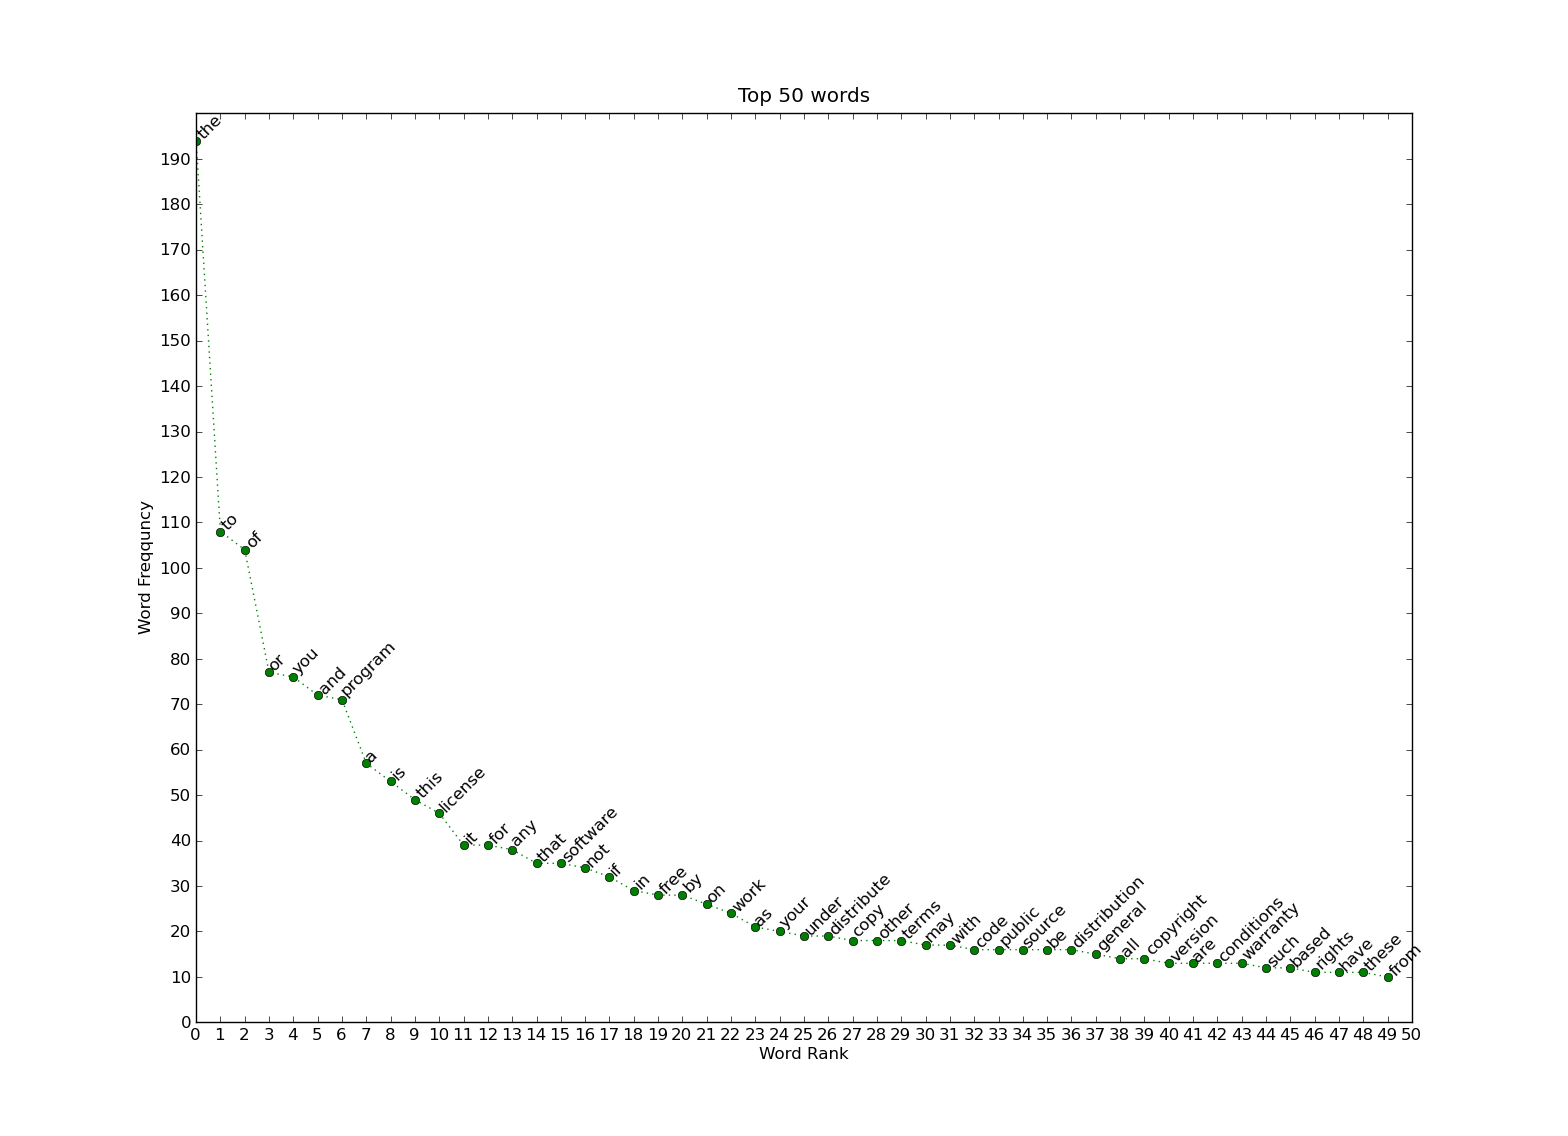
\includegraphics[height=8cm]{freq_tag.png}
\end{frame}

\begin{frame}[fragile]
 \frametitle{Plotting histogram of top N words}
Python code to plot histogram of top 50 words
\footnotesize
\begin{verbatim}
import numpy as np
import matplotlib.pyplot as plt

def plot_hist(text):
    tw = top_words(text)
    words = [tw[i][0] for i in range(len(tw))]
    freq = [tw[j][1] for j in range(len(tw))]
    pos = np.arange(len(words))
    width = 1.0
    ax = plt.axes(frameon=True)
    ax.set_xticks(pos)
    ax.set_yticks(range(0,max(freq),10))
    ax.set_xticklabels(words,rotation='vertical',fontsize=9)
    plt.bar(pos,freq,width, color='b')
    plt.show()

text = open('gpl-2.0.txt','r').read()
plot_hist(text)
\end{verbatim}

\end{frame}


\begin{frame}
 \frametitle{Histogram}
\small{Histogram of top 50 words from GPL v.2. (without filtering stop words)} \\
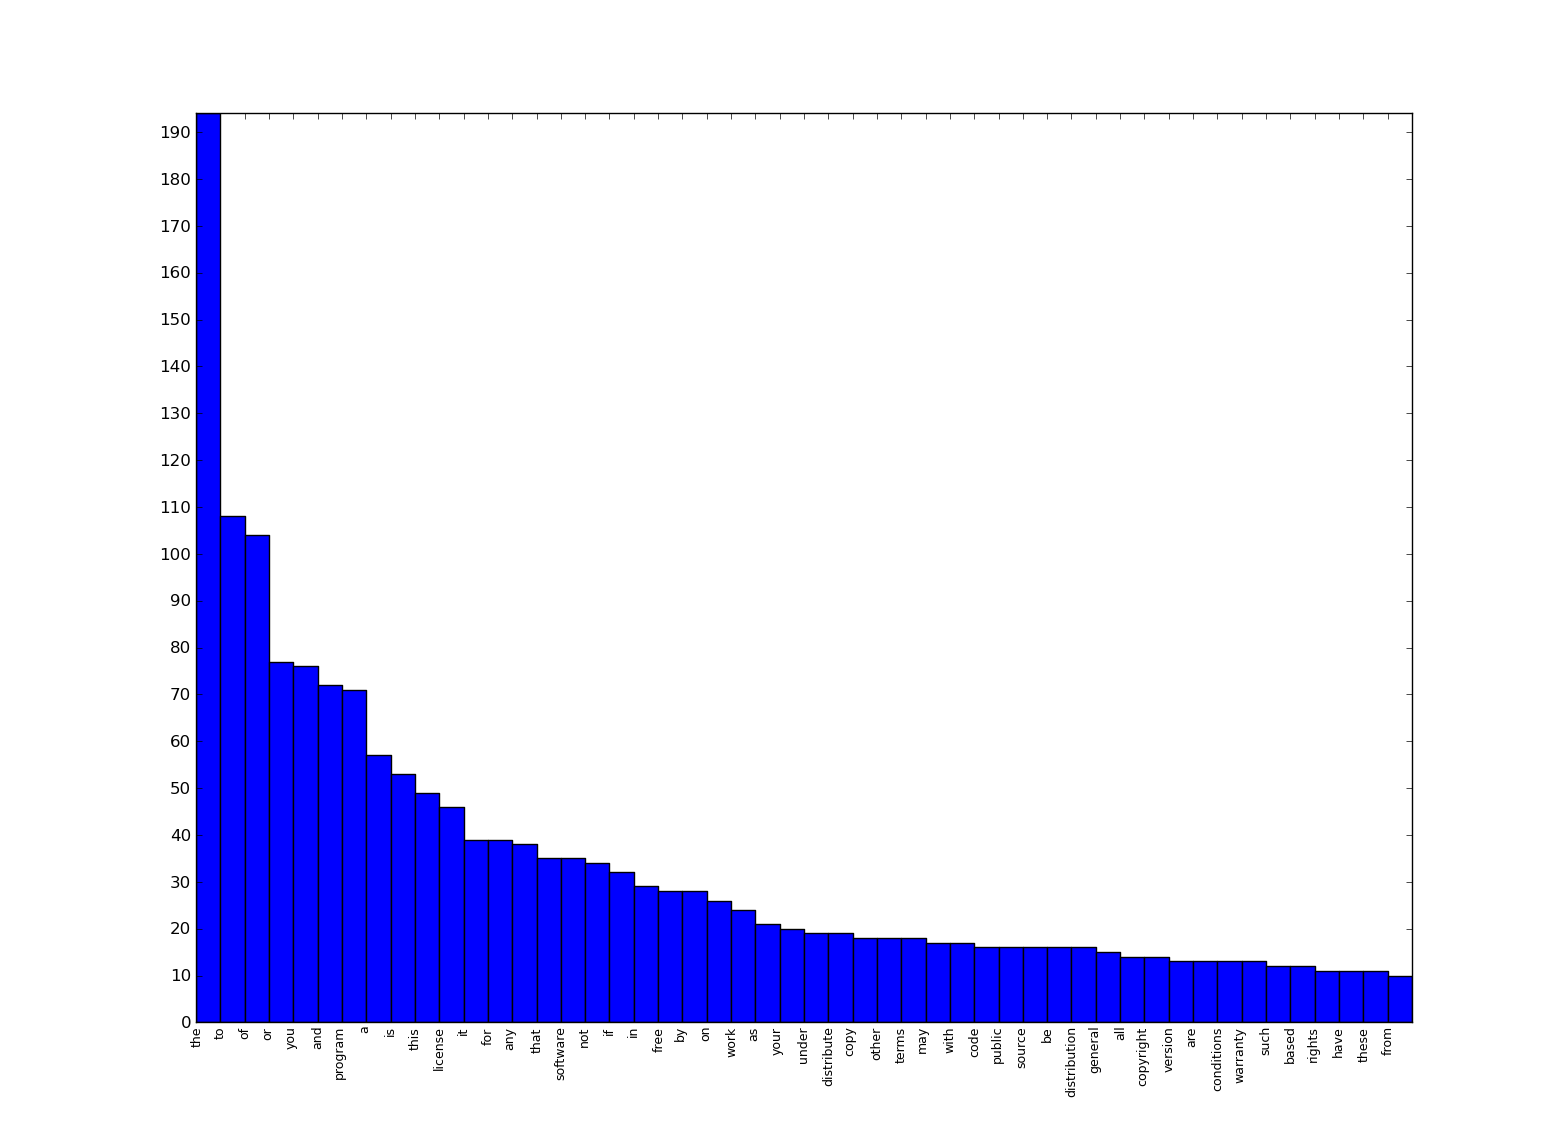
\includegraphics[height=8cm]{histogram.png}
\end{frame}


\begin{frame}[fragile]
 \frametitle{Lexical Dispersion Plot}
A lexical dispersion plot shows position of a word in given text. I have created some Python code to generate lexical dispersion plot with reference to a given word list\footnote{Code taken from \url{http://nltk.googlecode.com/svn/trunk/doc/api/nltk.draw.dispersion-pysrc.html} and modified}.
\tiny
\begin{verbatim}
def dispersion_plot(text,words):
    wordst = tokenize(text)
    points = [(x,y) for x in range(len(wordst))\
    for y in range(len(words)) if wordst[x] == words[y]]

    if points:
        x,y = zip(*points)
    else:
        x = y = ()

    plt.plot(x,y,"go",scalex=.2)
    plt.yticks(range(len(words)),words,color="b")
    plt.ylim(-1,len(words))
    plt.title("Lexical Dispersion Plot")
    plt.xlabel("Word Offset")
    plt.show()

gpl = open('gpl-2.0.txt','r').read()
dispersion_plot(gpl,['software','license','copy','gnu','program','free'])
\end{verbatim}

\end{frame}


\begin{frame}[fragile]
 \frametitle{Lexical Dispersion Plot}
\small
Lexical Dispersion Plot plot from GPL text \\
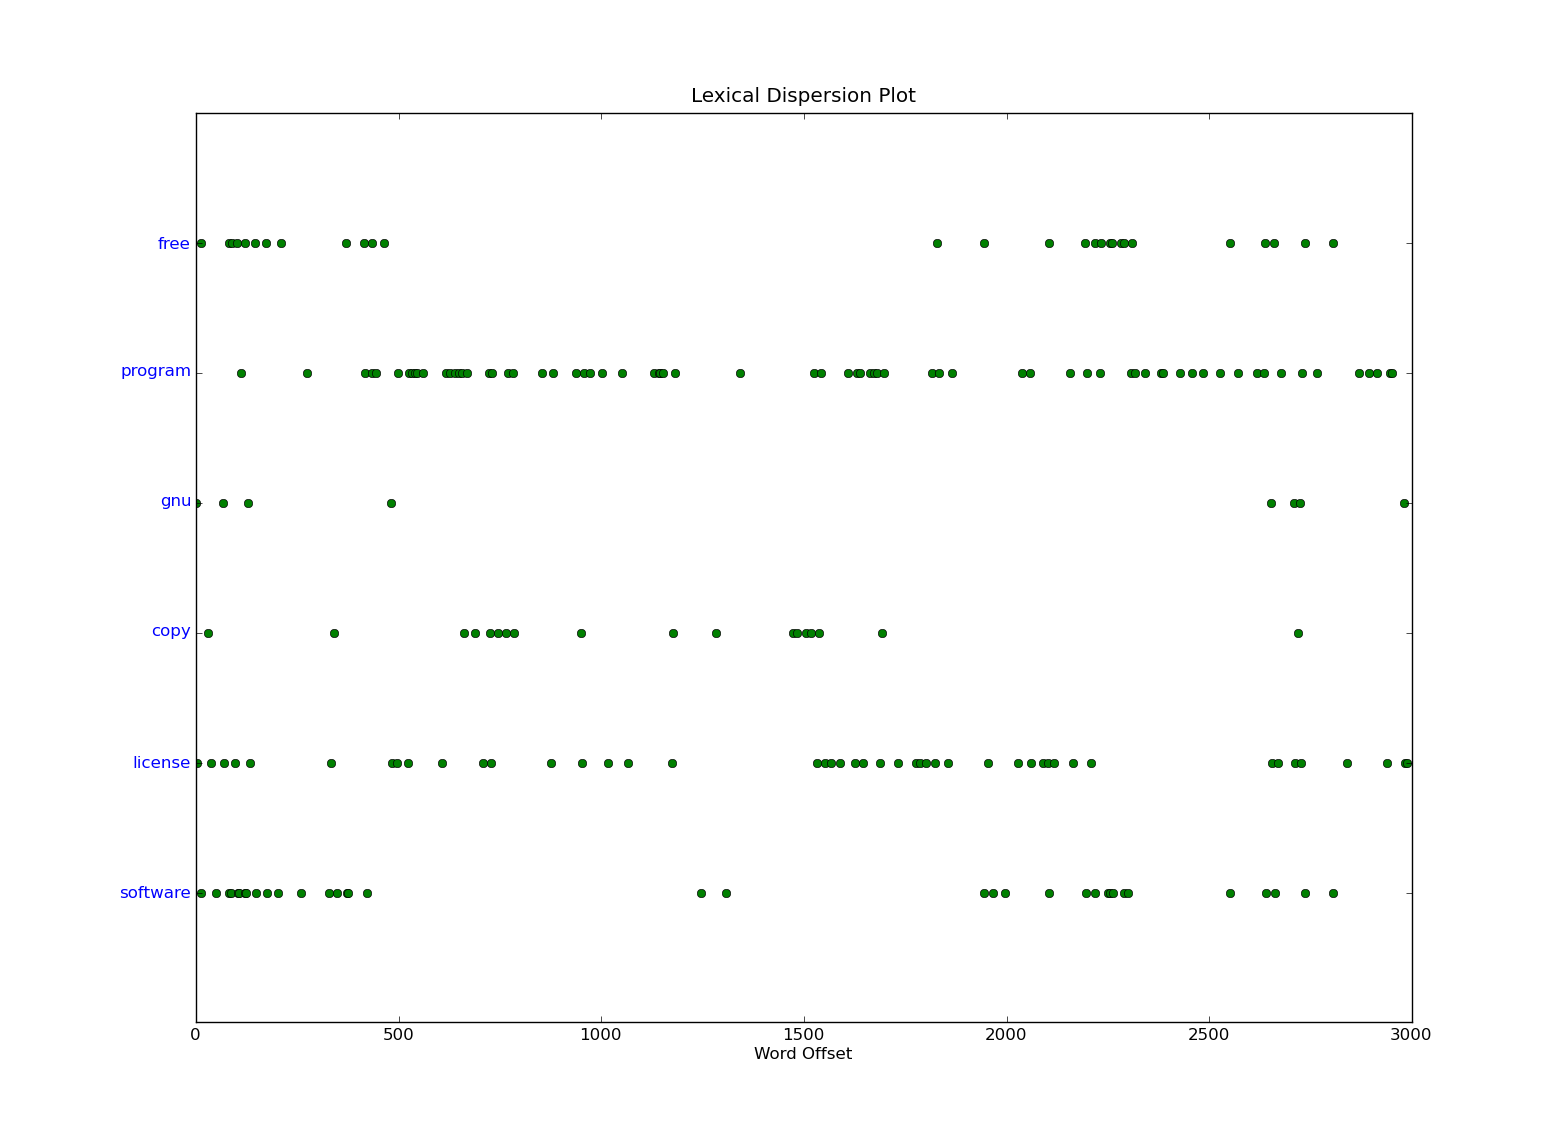
\includegraphics[height=8cm]{ld.png}
\end{frame}


\begin{frame}[fragile]
 \frametitle{Tag Cloud}
\small
A tag cloud (word cloud, or weighted list in visual design) is a visual representation for text data, typically used to depict keyword meta-data (tags) on websites, or to visualize free form text.
There is an interesting python tool to generate tag clouds from text called pytagcloud \footnote{\url{https://github.com/atizo/PyTagCloud}}. here comes an example of creating tag cloud from first 100 words from GPL text. 
\footnotesize
\begin{verbatim}
from pytagcloud import create_tag_image, make_tags
from pytagcloud.lang.counter import get_tag_counts

def create_tag_cloud(text):
    words = tokenize(text)
    doc = " ".join(d for d in words[:100])
    tags = make_tags(get_tag_counts(doc), maxsize=80)
    create_tag_image(tags, 'gpl.png', size=(900, 600), \
    fontname='Philosopher')

gpl = open('gpl-2.0.txt','r').read()
create_tag_cloud(gpl)
\end{verbatim}

\end{frame}

\begin{frame}[fragile]
 \frametitle{Tag Cloud}
Tag cloud from GPL text\\
\begin{center}
 
\includegraphics[height=6cm]{tc.png}
\end{center}

\end{frame}

\begin{frame}[fragile]
  \frametitle{Word co-occurrence}
Word co-occurrence analysis is used to construct lexicon ontologies etc.. In general it aims to find similarities between word pairs.
\begin{block}<+->{}
A word co-occurrence matrix is a square of $N \times N$ matrix where $N$ corresponds total number of unique words in a corpus. A cell $m_{ij}$ contains the number of times $m_{i}$ co-occur with word $m_{j}$ with in a specific context— a natural unit such as a sentence or a certain window of $m$ words. Note that the upper and lower triangles of the matrix are identical since co-occurrence is a symmetric relation. \footnote{Jimmy Lin,Scalable Language Processing Algorithms for the Masses: A Case Study in Computing Word Co-occurrence Matrices with MapReduce, \url{www.aclweb.org/anthology/D08-1044}}
\end{block}

\end{frame}

\begin{frame}[fragile]
 \frametitle{Word co-occourance}

\begin{center}
 \begin{tabular}{|l|l|l|l|l|l|}
 \hline
  & $w_{1}$ & $w_{2}$ & $w_{3}$ & .. & $w_{n}$ \\ \hline
 $w_{1}$ & $m_{11}$ & $m_{12}$ & $m_{13}$ & ..  & $m_{1n}$ \\ \hline
 $w_{2}$ & $m_{21}$ & $m_{22}$ & $m_{23}$ & ..  & $m_{2n}$ \\ \hline
 $w_{3}$ & $m_{31}$ & $m_{32}$ & $m_{33}$ & ..  & $m_{3n}$ \\ \hline
 .. & .. & .. & .. & ..  & .. \\ \hline
 $w_{n}$ & $m_{n1}$ & $m_{n2}$ & $m_{n3}$ & ..  & $m_{nn}$ \\ \hline
\end{tabular}
\scriptsize
\\ Shape of a co-occurrence matrix
\end{center}

\scriptsize

\end{frame}

\begin{frame}[fragile]
 \frametitle{Word co-occurrence}
Finding co-occurrence matrix with Python
\footnotesize
\begin{verbatim}
def cooccurrence_matrix_corpus(corpus):
    matrix = defaultdict(lambda : defaultdict(int))

    for corpora in corpus:
        for i in xrange(len(corpora)-1):
            for j in xrange(i+1, len(corpora)):
                word1, word2 = [corpora[i],corpora[j]]
                matrix[word1][word2] += 1
                matrix[word2][word1] += 1

    return matrix

corpus = [['w1','w2','w3'],['w4','w5','w6']]
ccm = cooccurrence_matrix_corpus(corpus)
\end{verbatim}

\end{frame}


\begin{frame}[fragile]
\frametitle{Word co-occurrence}
\begin{center}
 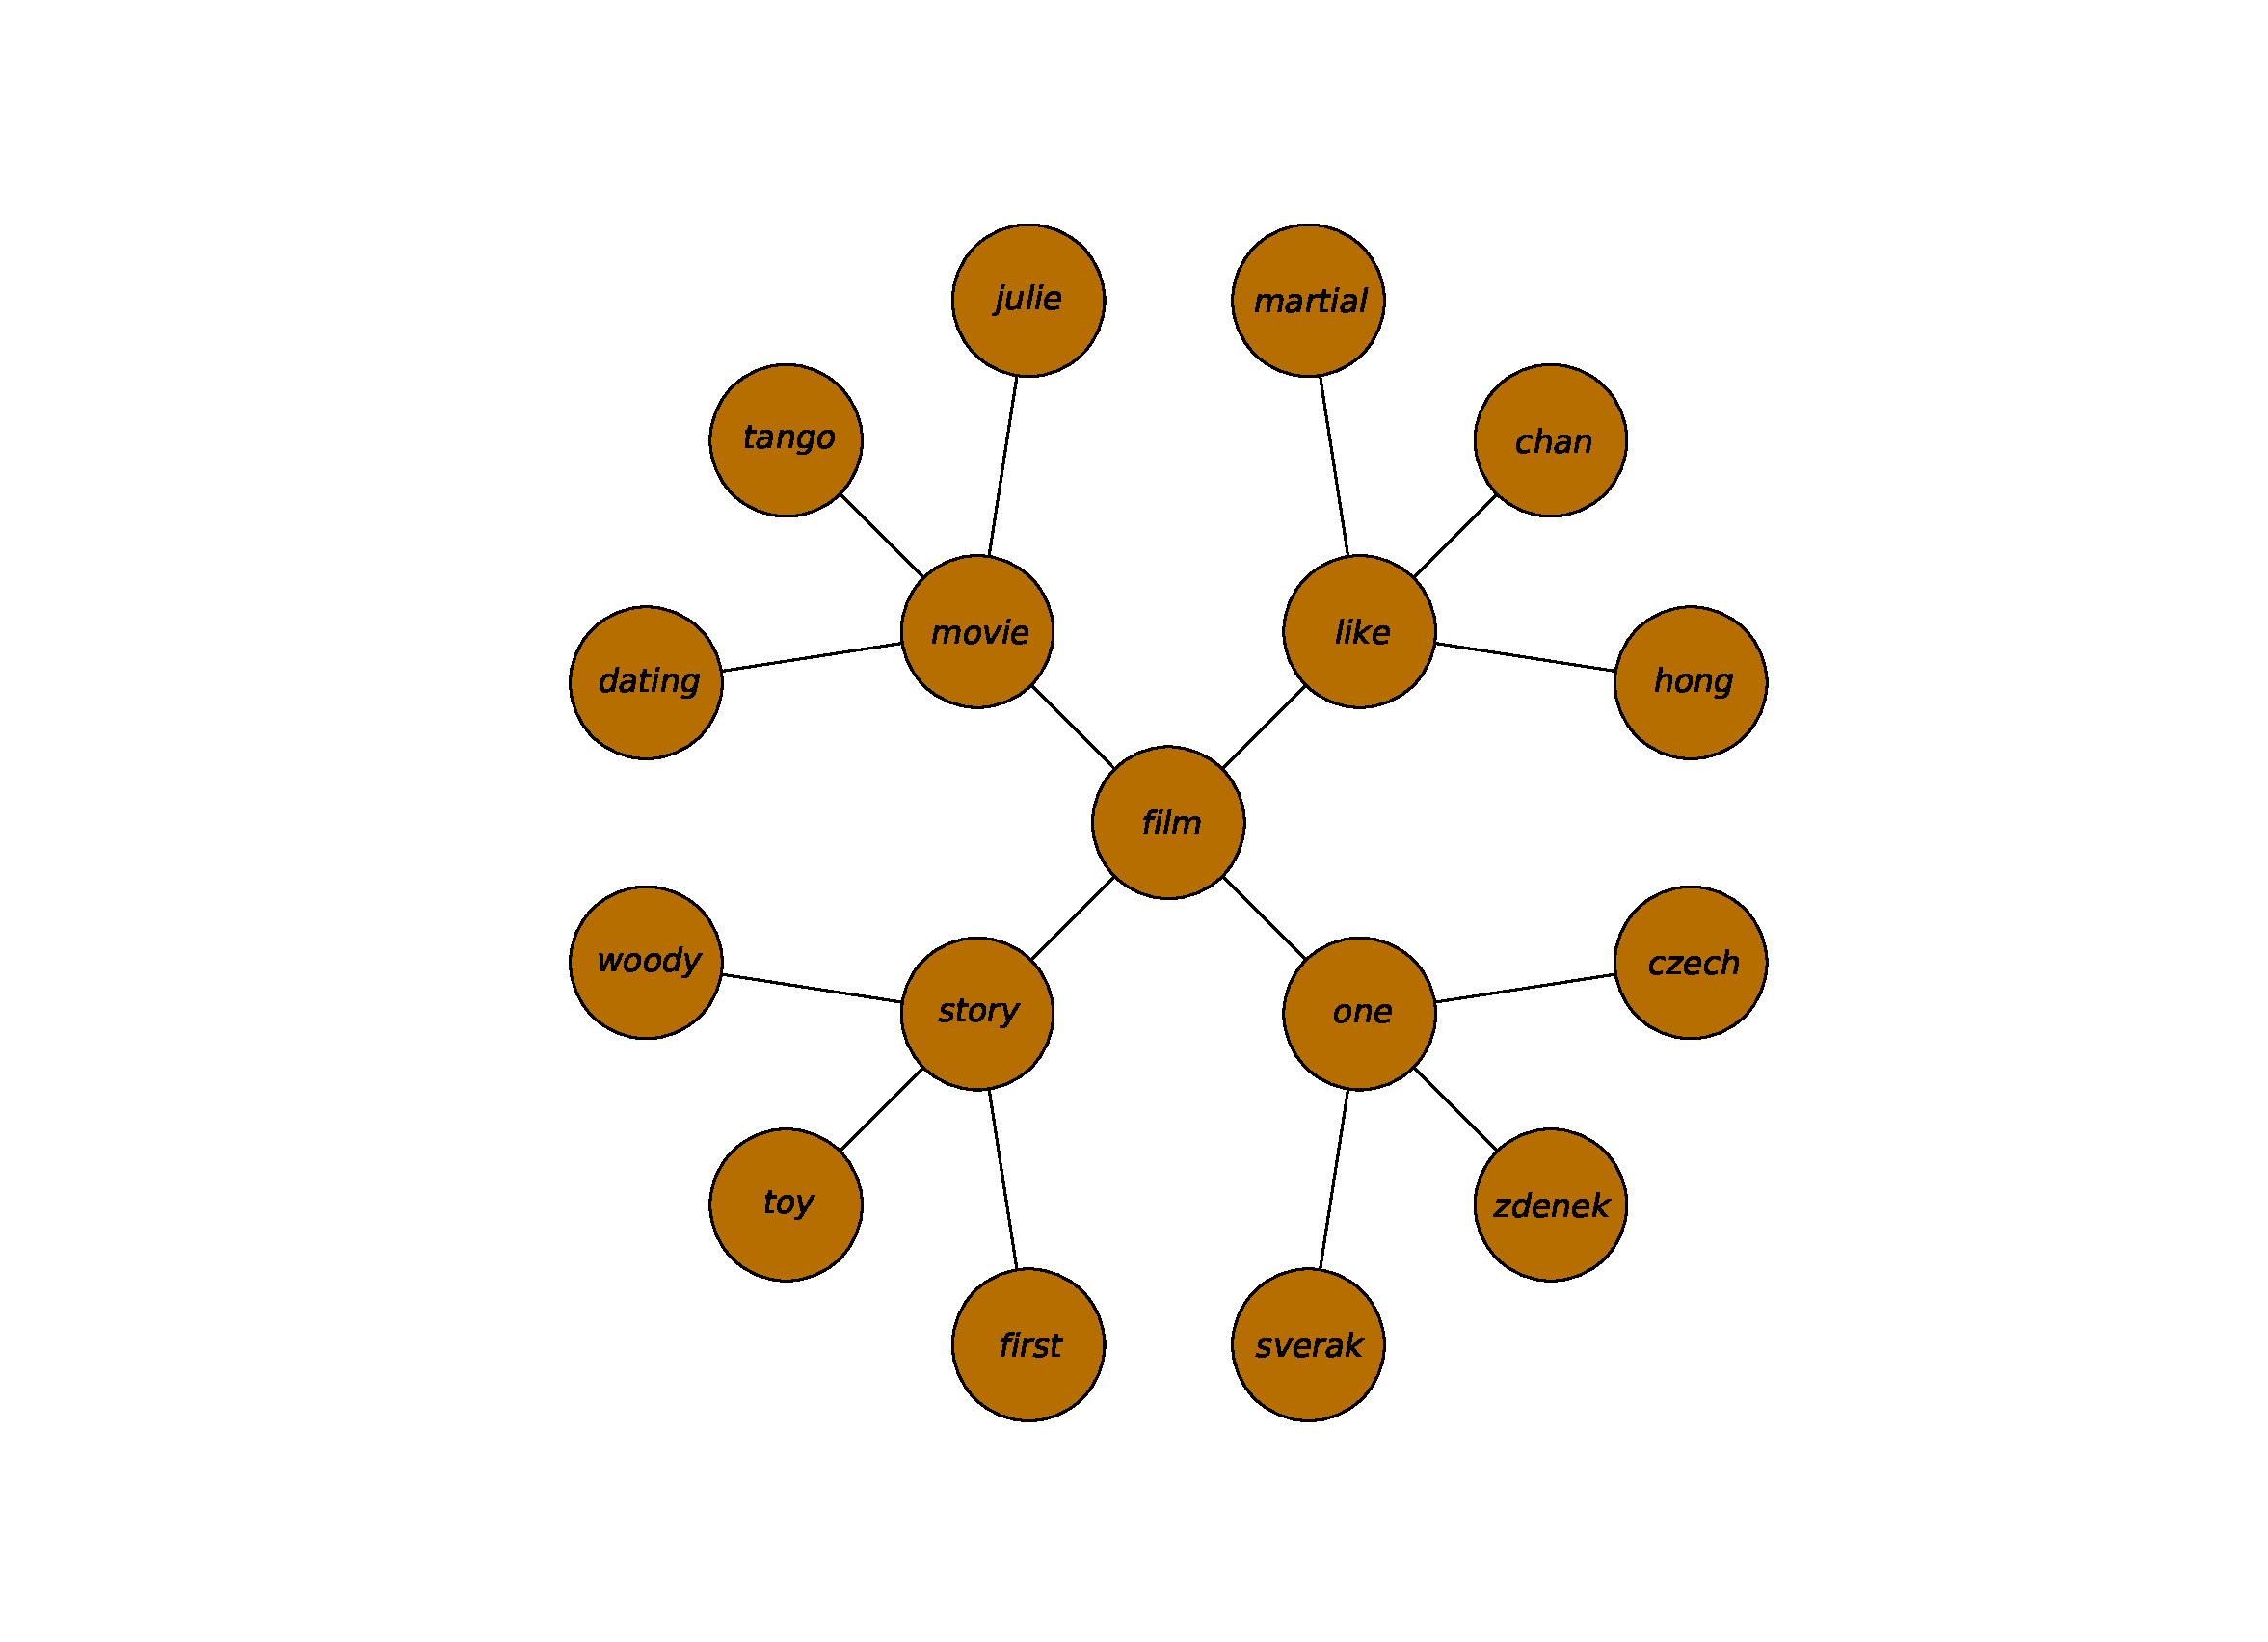
\includegraphics[height=6cm]{mov_rev_100_pos.pdf} 
\end{center}
\scriptsize
Word co-occurrence visualization from 100 positive movie reviews. The plot show top first word and top four associated words. For each associated words again associated words are plotted. 
\end{frame}


\begin{frame}[fragile]
 \frametitle{Stop Words}
\begin{block}<+->{Stop Words}
 In computing, stop words are words which are filtered out prior to, or after, processing of natural language data (text).
 In terms of linguistics these words are called as function words. Words like 'a', 'an', 'the' are examples for stop words. There is no defined set of stop words available. Different applications and research groups uses different sets o stop words. \\
 Generally stop words are omitted in text mining process. The frequency of stop words will be very high in any corpus compared to content words.Pointers to some good stop word list is available at \url{http://en.wikipedia.org/wiki/Stop_words}
\end{block}

\end{frame}


\begin{frame}[fragile]
 \frametitle{Stop Words Filter}
\tiny
\begin{verbatim}
def stop_filter(words):
    stops = ['i', 'me', 'my', 'myself', 'we', 'our', 'ours', 'ourselves', 'you', \
    'your', 'yours', 'yourself', 'yourselves', 'he', 'him', 'his', 'himself', 'she',\
    'her', 'hers', 'herself', 'it', 'its', 'itself','they', 'them', 'their', 'theirs',\
    'themselves', 'what', 'which', 'who', 'whom', 'this', 'that', 'these', 'those', \
    'am', 'is', 'are', 'was', 'were','be', 'been', 'being', 'have', 'has', 'had', \
    'having', 'do', 'does', 'did', 'doing', 'a', 'an', 'the', 'and', 'but', 'if', 'or', 'because',\
    'as', 'until', 'while', 'of', 'at', 'by', 'for','with', 'about', 'against', 'between', 'into', \
    'through', 'during', 'before', 'after', 'above', 'below', 'to', 'from', 'up', 'down', 'in', 'out',\
    'on', 'off', 'over', 'under', 'again', 'further','then', 'once', 'here', 'there', 'when', 'where', \
    'why', 'how', 'all', 'any', 'both', 'each', 'few', 'more', 'most', 'other', 'some', 'such', 'no',\
    'nor','not', 'only', 'own', 'same', 'so', 'than', 'too', 'very', 's', 't', 'can', 'will', 'just',\
    'don', 'should', 'now']

    stopless = [word in words if word not in stops]
    
    return stopless
\end{verbatim}

\end{frame}


\begin{frame}[fragile]
 \frametitle{Bag of Words}

\begin{block}<+->{}
 The bag-of-words model is a simplifying representation used in natural language processing and information retrieval (IR). In this model, a text (such as a sentence or a document) is represented as an un-ordered collection of words, disregarding grammar and even word order. \footnote[]{http://en.wikipedia.org/wiki/Bag\_of\_words\_model} \\
 Analyzing text by only analyzing frequency of words is called as bag of words model.
\end{block}

\end{frame}

\begin{frame}[fragile]
 \frametitle{Bag of Words}
 %\framebox[1]
\begin{block}<+->{Example}
\begin{Verbatim}[frame=single]
 d1: John likes to watch movies. Mary likes too.
 d2: John also likes to watch football games.
\end{Verbatim}

\begin{Verbatim}[frame=single]
 {'football': 0, 'watch': 6, 'movies': 5, 'games': 1, 
 'likes': 3, 'john': 2, 'mary': 4}
  * after removing stopwords 
\end{Verbatim}

\begin{Verbatim}[frame=single]
 [0, 0, 1, 2, 1, 1, 1]
 [1, 1, 1, 1, 0, 0, 1]
each entry of the vectors refers to count of 
the corresponding entry in the dictionary
\end{Verbatim}
\footnote{Example taken from http://en.wikipedia.org/wiki/Bag\_of\_words\_model }
\end{block}

\end{frame}

\begin{frame}[fragile]
 \frametitle{Bag of Words}
 \begin{block}<+->{Documents}
  \begin{Verbatim}[frame=single]
 d1: John likes to watch movies. Mary likes too.
 d2: John also likes to watch football games.
  \end{Verbatim}
  \end{block}

 \begin{block}<+->{Vocabulary Index}
  \begin{displaymath}
  VI(t) = \left\{ 
 \begin{array}{l l l l l l l} 
  0, & \quad \text{if t is 'football'} \\
  1, & \quad \text{if t is  'games'} \\
  2, & \quad \text{if t is 'john'} \\
  3, & \quad \text{if t is 'likes'} \\
  4, & \quad \text{if t is  'mary'} \\ 
  5, & \quad \text{if t is 'movies'} \\ 
  6, & \quad \text{if t is 'watch'} \\
 \end{array}\right.
 \end{displaymath}

 \end{block}

\end{frame}

\begin{frame}[fragile]
 \frametitle{Bag of Words}
  \begin{tabular}{|l|l|l|l|l|l|l|l|}
  \hline
   & football & games & john & likes & mary & movies & watch \\ \hline
  doc1 & 0 & 0 & 1 & 2 & 1 & 1 & 1 \\ \hline
  doc2 & 1 & 1 & 1 & 1 & 0 & 0 & 1 \\
  \hline
  \end{tabular}
\end{frame}


\begin{frame}[fragile]
 \frametitle{Bag of Words}
Creating Bag of Words with Python and sklearn \footnote{http://scikit-learn.org}
\footnotesize
\begin{Verbatim}[frame=single]
 from sklearn.feature_extraction.text import\
 CountVectorizer
 vectorizer = CountVectorizer(analyzer='word',\
 min_n=1,stop_words='english')
 docs = ('John likes to watch movies. Mary \
 likes too.','John also likes to watch football games.')
 bow = vectorizer.fit_transform(docs)
 print vectorizer.vocabulary_
 print bow.toarray()
\end{Verbatim}

\end{frame}

\begin{frame}[fragile]
 \frametitle{Bag of Words}
Creating Bag of Words with Python. Just for sample ;-(
\footnotesize
\begin{verbatim}

def bag_of_words(docs):
    stops = ['to','too','also']
    token_list = [tokenize(doc) for doc in docs]
    vocab = list(set(token_list[0]).union(*token_list))
    vocab =[v for v in vocab if v not in stops and len(v) > 1]
    vocab_idex = dict( [ ( word, vocab.index(word) ) for word \
    in vocab] )
    bow = [[tokens.count(word) for word in vocab_idex.keys()] \
    for tokens in token_list]
    print vocab_idex
    for bag in bow:
        print bag

d = ("John likes to watch movies. Mary likes too.",\
"John also likes to watch football games.")

bag_of_words(d)
\end{verbatim}

\end{frame}


\begin{frame}[fragile]
 \frametitle{TF-IDF}
Tf–idf, term frequency–inverse document frequency, is a numerical statistic which reflects how important a word is to a document in a collection or corpus. 
\begin{block}<+-> {TF-IDF}
\begin{displaymath}
 tf-idf(t) = tf(t,d) \times idf(t)
\end{displaymath}
where 't' is a term in document 'd' \\
$tf(t,d)$ : how many times the term 't' is present in 'd'
 \begin{displaymath}
  tf(t,d) = \sum_{ x \in d} fr(x,t)
 \end{displaymath}

where
\begin{displaymath}
 fr(x,t) = \left\{
  \begin{array}{l l} 
   1, & \quad \text{if x = t} \\
   0, & \quad \text{otherwise} \\
  \end{array} \right.
\end{displaymath}

 %tf(t,d) : how many times the term 't' is present in 'd'
  %\begin{displaymath}
   %tf('john',d1) = 1 
   %\end{displaymath}
\end{block}

\end{frame}

\begin{frame}[fragile]
 \frametitle{TF-IDF}
 \begin{block}<+->{TF-IDF}
 and \\
  $idf(t) = log \frac{|D|}{1+|\{d : t \in d\}|}$ \\
 where $  | \{d : t \in d\} | $ is    $count(d)$ where 't' is present and $tf(t,d) \ne 0$ \\
 $|D|$ is the cardinality of the document space
 \end{block}

\end{frame}



\begin{frame}[fragile]
 \frametitle{TF}
 \begin{block}<+->{TF}
   \begin{displaymath}
    tf(t,d) = \sum_ { x \in d} fr(x,t)  
   \end{displaymath}

  $fr(x,t)$ is a simple function\\
  $fr(x,t) = \left\{
  \begin{array}{l l} 
   1, & \quad \text{if x = t} \\
   0, & \quad \text{otherwise} \\
  \end{array} \right. $ \\
  Example \\
  $tf('john',d1) = 1 $
 \end{block}

\end{frame}


\begin{frame}[fragile]
 \frametitle{Document Vector}
 \begin{block}<+->{}

To create a document vector space \\
\begin{displaymath}
 V\vec{d}_{n} = (tf({t}_1,{d}_n),tf({t}_2,{d}_n),,,,tf({t}_n,{d}_n))
\end{displaymath}
To represent 'd1' and 'd2' as vectors 
\footnotesize
\begin{displaymath}
 V\vec{d}_{1} = (tf({t}_1,{d}_1),tf({t}_2,{d}_1),tf({t}_3,{d}_1),tf({t}_4,{d}_1),tf({t}_5,{d}_1),tf({t}_6,{d}_1),tf({t}_7,{d}_1))
 \end{displaymath}
 \footnotesize
\begin{displaymath}
 V\vec{d}_{2} = (tf({t}_1,{d}_2),tf({t}_2,{d}_2),tf({t}_3,{d}_2),tf({t}_4,{d}_2),tf({t}_5,{d}_2),tf({t}_6,{d}_2),,tf({t}_7,{d}_2))
\end{displaymath}
which evaluates to 
\begin{displaymath}
 V\vec{d}_{1} = (0, 0, 1, 2, 1, 1, 1)
\end{displaymath}

\begin{displaymath}
 V\vec{d}_{2} = (1, 1, 1, 1, 0, 0, 1)
\end{displaymath}

 \end{block}

\end{frame}

\begin{frame}[fragile]
 \frametitle{Vector Space Matrix}
\begin{block}<+->{}
 The document vectors can be represented as matrix
 \begin{displaymath}
  M_{|D|  x  F }
  \end{displaymath}
  where $|D|$ is the cardinality of the document space
  \begin{displaymath}
  M_{|D|   x  F }  = \begin{bmatrix}
                    0 & 0 & 1 & 2 & 1 & 1 & 1 \\

                    1 & 1 & 1 & 1 & 0 & 0 & 1
                   \end{bmatrix}
  \end{displaymath}
  \end{block}

\end{frame}

\begin{frame}[fragile]
 \frametitle{Vector Normalization}
 \begin{block}<+->{Normalized Vector}
  A normalized vector is represented as
  %V\vec{d}_{1} = [0, 0, 1, 2, 1, 1, 1]
  %\begin{displaymath}
   $\hat{v} = \frac{\vec{v}}{\|\vec{v}\|_p}$
  %\end{displaymath}
where $\hat{v}$ is is the unit vector, or the normalized vector, the $\vec{v}$ is the vector going to be normalized and the $\|\vec{v}\|_p$ is the norm (magnitude or length) of the vector $\vec{v}$ in the $L^{P}$ space (Lebesgue spaces) \footnote{http://en.wikipedia.org/wiki/Lp\_space}.
 \end{block}

\end{frame}

\begin{frame}[fragile]
 \frametitle{Vector Normalization}
 % $ V\vec d_{1} = [0, 0, 1, 2, 1, 1, 1] $
Length of a vector is calculated using the Euclidean norm \footnote{http://mathworld.wolfram.com/L2-Norm.html}. \\
%The non-normalized term frequency vector of document $ d_{1} $ is $ V\vec d_{1} = [0, 0, 1, 2, 1, 1, 1] $ \\
Non-normalized vector  $\vec v = (v_{1},v_{2},v_{3},...v_{n}) $ \\ 
Length of vector $ \|\vec v \| = \sqrt {v_{1}^{2} + v_{2}^{2} + v_{2}^{2} + ... + v_{n}^{2}} $ \\ 
With norm $ \| \vec v || _{p} = (|v_{1}|^{p} + |v_{2}|^{p} + |v_{3}|^{p} + ... + |v_{n}|^{p})^\frac{1}{p} $ \\
It can be simplified as\\ 
\begin{displaymath}
 \| \vec v || _{p} = ( \sum_{i=1}^{n} |\vec v_{i}| ^{p}) ^{ \frac{1}{p}}
\end{displaymath}

\end{frame}

\begin{frame}[fragile]
 \frametitle{Vector Normalization}
\begin{block}<+->{L2 Norm}
 The norm which we apply here is L2 Norm which is also called as Euclidean norm \footnote{http://en.wikipedia.org/wiki/Norm\_(mathematics)\#Euclidean\_norm} \\
It is a common norm used to measure the length of a vector where $p = 2 $
\end{block}

\end{frame}

\begin{frame}[fragile]
 \frametitle{Vector Normalization}
$ v\vec d_{1} = (0, 0, 1, 2, 1, 1, 1) $ \\
$ \hat{v} d_{1} = \frac{\vec v}{\|\vec v \| _{p}} $ \\
$ \hat{v}d_{1} = \frac{v \vec d_{1}} {\|v\vec d_{1} \| _{2}} $ \\
$ \hat{v}d_{1} = \frac{(0, 0, 1, 2, 1, 1, 1)}{\sqrt{0^{2} + 0^{2} + 1^{2} + 2^{2} + 1^{2} + 1^{2} + 1^{2}}} $ \\
$ \hat{v}d_{1} = \frac{(0, 0, 1, 2, 1, 1, 1)}{\sqrt{8}} $ \\
$ \hat{v}d_{1} = (\frac{0}{\sqrt{8}},\frac{0}{\sqrt{8}},\frac{1}{\sqrt{8}},\frac{2}{\sqrt{8}},\frac{1}{\sqrt{8}},\frac{1}{\sqrt{8}},\frac{1}{\sqrt{8}}) $ \\
$ \hat{v}d_{1} = (0.0, 0.0, 0.3535, 0.7071, 0.3535, 0.3535, 0.3535)$ \\
Now our normalized vector $\hat{v}d_{1}$ has now a L2-norm $\| \hat{v}d_{1} \| _{2} = 1.0 $
\end{frame}



\begin{frame}[fragile]
 \frametitle{IDF}
\begin{block}<+->{IDF}
 %\begin{displaymath}
  $idf(t) = log \frac{|D|}{1+|\{d : t \in d\}|}$ \\
 %\end{displaymath}
%\begin{displaymath}
 %\[ 
 where $  | \{d : t \in d\} | $ is    $count(d)$ where 't' is present and $tf(t,d) \ne 0$
%\]
%\end{displaymath}

\end{block}

\end{frame}

\begin{frame}[fragile]
 \frametitle{Finding IDF}
\begin{block}<+->{}
 \begin{displaymath}
  idf(t_{i}) = log \frac{|D|}{1+|\{d : t_{i} \in d\}|} = log \frac{2}{1} = 0.69314718
 \end{displaymath}
\footnotesize
$idf(football) = log \frac{2}{1+1} = 0.0 $ \\
$idf(games) = log \frac{2}{1+1} = 0.0 $ \\
$idf(john) = log \frac{2}{1+2} = -0.40546510810816444 $ \\
$idf(likes) = log \frac{2}{1+2} = -0.40546510810816444 $ \\
$idf(mary) = log \frac{2}{1+1} = 0.0 $ \\
$idf(movies) = log \frac{2}{1+1} = 0.0 $ \\
$idf(watch) = log \frac{2}{1+1} = 0.0 $ \\
%\begin{displaymath}
 %\text{IDF of V = } 
$idf(V)$ = (0.,0.,-0.40546510810816444,-0.40546510810816444,0.0,0.0,0.0)
%\end{displaymath}

\end{block}

\end{frame}

%\begin{frame}[fragile]
% \frametitle{Finding IDF}

%\end{frame}

\begin{frame}[fragile]
 \frametitle{TF-IDF weight}
\begin{block}<+->{Finding TF-IDF weight}
 \begin{displaymath}
  M_{|D|  \times F } \quad \times \quad M_{idf}
 \end{displaymath}

\end{block}
\begin{block}<+->{}
 \footnotesize
 \begin{displaymath}
  \begin{bmatrix}
 tf(t_{1},d_{1}) & tf(t_{2},d_{1}) & tf(t_{3},d_{1}) & tf(t_{4},d_{1}) & tf(t_{5},d_{1}) & tf(t_{6},d_{1}) & tf(t_{7},d_{1}) ) \\

 tf(t_{1},d_{2}) & tf(t_{2},d_{2}) & tf(t_{3},d_{2}) & tf(t_{4},d_{2}) & tf(t_{5},d_{2}) & tf(t_{6},d_{2}) & tf(t_{7},d_{2}))
  \end{bmatrix}
  \end{displaymath}
 x
  \footnotesize
\begin{displaymath}
  \begin{bmatrix}
   idf(t_{1}) & 0 & 0 & 0 & 0 & 0 & 0 \\

   0 & idf(t_{2}) & 0 & 0 & 0 & 0 & 0 \\

   0 & 0 & idf(t_{3}) & 0 & 0 & 0 & 0 \\

   0 & 0 & 0 & idf(t_{4}) & 0 & 0 & 0 \\

   0 & 0 & 0 & 0 & idf(t_{5}) & 0 & 0 \\
   
   0 & 0 & 0 & 0 & 0 & idf(t_{6}) & 0 \\
   
   0 & 0 & 0 & 0 & 0 & 0 & idf(t_{6})
  \end{bmatrix}
\end{displaymath}


\end{block}

\end{frame}

\begin{frame}[fragile]
 \frametitle{TF-IDF weight}
\footnotesize
\begin{displaymath}
 \begin{bmatrix}
  tf(t_{1},d_{1}) \times idf(t_{1}) & tf(t_{2},d_{1}) \times idf(t_{2}) & tf(t_{3},d_{1}) \times idf(t_{3}) & \\
tf(t_{4},d_{1}) \times idf(t_{4} & tf(t_{5},d_{1}) \times idf(t_{5} & tf(t_{6},d_{1}) \times idf(t_{6} & tf(t_{7},d_{1}) \times idf(t_{7}) \\
 tf(t_{1},d_{2}) \times idf(t_{1}) & tf(t_{2},d_{2}) \times idf(t_{2}) & tf(t_{3},d_{2}) \times idf(t_{3}) & \\
tf(t_{4},d_{2}) \times idf(t_{4} & tf(t_{5},d_{2}) \times idf(t_{5} & tf(t_{6},d_{2}) \times idf(t_{6} & tf(t_{7},d_{2}) \times idf(t_{7})
 \end{bmatrix}
\end{displaymath}

\end{frame}


\begin{frame}[fragile]
 \frametitle{TF-IDF Normalization}
  \begin{block}<+-> { L2 Normalization }
  \begin{displaymath}
  M_{tf-idf} = \frac{M_{tf-idf}}{\|M_{tf-idf}\| _{2}}
  \end{displaymath}

  \end{block}

\end{frame}

\begin{frame}[fragile]
 \frametitle{TF-IDF}
Practice with Python and sklearn \footnote{http://scikit-learn.org}
\footnotesize
\begin{Verbatim}[frame=single]
 from sklearn.feature_extraction.text import\
 CountVectorizer, TfidfTransformer
 vectorizer = CountVectorizer(analyzer='word',\
 min_n=1,stop_words='english')
 docs = ('John likes to watch movies. Mary \
 likes too.','John also likes to watch football games.')
 bow = vectorizer.fit_transform(docs)
 freq_term_matrix =vectorizer.transform(docs)
 tfidf = TfidfTransformer(norm="l2")
 tfd = tfidf.fit(freq_term_matrix)
 print "IDF:", tfidf.idf_
 tf_idf_matrix = tfidf.transform(freq_term_matrix)
 print tf_idf_matrix.todense()
 for w,f in zip(vectorizer.vocabulary_,tfd.idf_):
  print '%r => %r' % (w, tfd.idf_[f])
\end{Verbatim}

\end{frame}


\begin{frame}[fragile]
 \frametitle{N-Grams}
\begin{block}<+->{N-Gram}
 In the fields of computational linguistics and probability, an n-gram is a contiguous sequence of n items from a given sequence of text or speech. An n-gram could be any combination of letters. However, the items in question can be phonemes, syllables, letters, words or base pairs according to the application.\footnote{http://en.wikipedia.org/wiki/N-gram} \\
 \begin{itemize}
  \item Unigrams are single words
  \item Bigrams are sequences of two words
  \item Trigrams are sequences of three words
 \end{itemize}

\end{block}

\end{frame}

\begin{frame}[fragile]
 \frametitle{Bigrams}
 \begin{block}<+->{Bigrams}
  $ P(w_{i}|w_{1},w_{2},...,w_{i-1})  \approx P(w_{i},w_{i-1})$
 \end{block}
 \begin{block}<+->{Practice with Python}
  \footnotesize
  \begin{Verbatim}
   d1 = "John likes to watch movies. Mary likes too."
   words = d1.lower().split()
   ibigrams = [words[x:x+2] for x in xrange(len(words)-2+1)]
   bigrams = [" ".join(bigram) for bigram in ibigrams]
   print bigrams

   ['john likes', 'likes to', 'to watch', 'watch movies.', \
   'movies. mary', 'mary likes', 'likes too.']
  \end{Verbatim}

 \end{block}

\end{frame}

\begin{frame}[fragile]
 \frametitle{Trigrams}
 \begin{block}<+->{Trigrams}
  $ P(w_{i}|w_{1},w_{2},...,w_{i-1})  \approx P(w_{i},w_{i-2},w_{i-1})$
 \end{block}
 \begin{block}<+->{Practice with Python}
  \footnotesize
   \begin{Verbatim}
    d1 = "John likes to watch movies. Mary likes too."
    words = d1.lower().split()
    itrigrams = [words[x:x+3] for x in xrange(len(words)-3+1)]
    trigrams = [" ".join(trigram) for trigram in itrigrams]
    print trigrams

    ['john likes to', 'likes to watch', 'to watch movies.', \
    'watch movies. mary', 'movies. mary likes', 'mary likes too.']
   \end{Verbatim}

 \end{block}


\end{frame}

\begin{frame}[fragile]
 \frametitle{N-Grams}
 Python code to generate N-Grams from list of words.
 \footnotesize
 \begin{Verbatim}

 def ngrams(words,n=2):
    grams = [" ".join(words[x:x+n]) for x in xrange(len(words)-n+1)]
    return grams

 words = "John likes to watch movies. Mary likes too."\
 .lower().split()
 bigrams = ngrams(words,n=2)
 trigrams = ngrams(words,n=3)
 print bigram
 print trigrams
 \end{Verbatim}

\end{frame}


\begin{frame}[fragile]
 \frametitle{Mutual Information}
\begin{block}<+->{Mutual Information}
 Statistical test to measure strength of word association \\
 $ I(w_{i},w_{j}) = log_{2}\frac{P(w_{i},w_{j})}{P(w_{i})P(w_{j})} \approx log_{2} \frac{NC(w_{i},w_{j})}{C(w_{i}) C(w_{j})} $ \\
 where $C(w_{i})$ and $C(w_{j})$ respective frequency of $w_{i}$ and $w_{j}$ in the corpus \\
 $C(w_{i},w_{j})$ is the frequency of bigram $w_{i},w_{j}$ \\
 $N$ is the total number of words in the corpus
\end{block}

\begin{block}<+->{}
 $ I(strong,tea) = log_{2}\frac{P(strong,tea)}{P(strong)P(strong)} \approx log_{2} \frac{NC(strong,tea)}{C(strong) C(tea)} $
\end{block}


\end{frame}


\begin{frame}[fragile]
 \frametitle{Mutual Information}
 \footnotesize
 \begin{verbatim}
from __future__ import division
import math

def mutual_info(words):
    grams = ngrams(words,n=2) #ngrams function from prev slide
    wordcount = {}
    gramcount = {}
    minfo = {}
    [ wordcount.__setitem__(word, 1 + \
    wordcount.get( word,0 )) for word in words ]
    [ gramcount.__setitem__(gram, 1 + \
    gramcount.get( gram,0 )) for gram in grams ]
    for gram in grams:
      minfo[gram] = (math.log( len(words) * gramcount[ gram ] \
      / wordcount[gram.split()[0]] * wordcount[ gram.split()[1]])) \
      / math.log( 2 )
    return minfo
\end{verbatim}
\end{frame}

\begin{frame}[fragile]
 \frametitle{t-score}
 \begin{block}<+->{t-score}
  Statistical test to measure strength of word association \\
  $ t(w_{i},w_{j}) = \frac{mean(P(w_{i},w_{j})) - mean(P(w_{i}) mean(P(w_{j})}{\sqrt{\sigma^{2}(P(w_{i},w_{j}) + \sigma^{2}(P(w_{i}) \sigma^{2}(P(w_{j})  ) }}$ \\
  %$\approx \frac{C(w_{i},w_{j}) - \frac{1}{N} C(w_{i}) C(w_{j})}{\sqrt{C(w_{i},w_{j})}}$ \\
  $\approx \frac{C(w_{i},w_{j}) - \frac{1}{N} C(w_{i}) C(w_{j})}{\sqrt{C(w_{i},w_{j})}}$ \\ %orig
  %$ \approx \frac{ \frac{C(w_{i},w_{j})}{N} - \frac{C(w_{i}}{N} \frac{C(w_{j}}{N}}{ \sqrt{ \frac{C(w_{i},w_{j})}{N^{2}} } }$ \\
  where $C(w_{i})$ and $C(w_{j})$ respective frequency of $w_{i}$ and $w_{j}$ in the corpus \\
 $C(w_{i},w_{j})$ is the frequency of bigram $w_{i},w_{j}$ \\
 $N$ is the total number of words in the corpus
 \end{block}

 \begin{block}<+->{}
  $ t(strong,tea) = \frac{C(strong,tea) - \frac{1}{N} C(strong) C(tea)}{\sqrt{C(strong,tea)}}$ \\
 %$ t(strong,tea) = \frac{ \frac{C(strong,tea)}{N} - \frac{C(strong)}{N} \frac{C(tea)}{N}}{ \sqrt{ \frac{C(strong,tea)}{N^{2}} } } $
 
 \end{block}
\end{frame}


\begin{frame}[fragile]
 \frametitle{t-score}
\footnotesize
\begin{verbatim}
 from __future__ import division
 import math

 def tscore(words):
   grams = ngrams(words,n=2) #ngrams function from prev slide
   wordcount = {}
   gramcount = {}
   tsc = {}
   [ wordcount.__setitem__(word, 1 + \
   wordcount.get( word,0 )) for word in words ]
   [ gramcount.__setitem__(gram, 1 + \
   gramcount.get( gram,0 )) for gram in grams ]
   for gram in grams:
      tsc[gram] =  (gramcount[gram]  - (1/len(words)) * \
      wordcount[gram.split()[0]]  * wordcount[gram.split()[1]])\
      / math.sqrt( gramcount[gram])
   return tsc
\end{verbatim}

\end{frame}


\begin{frame}[fragile]
 \frametitle{Document Classification}
Document classification or document categorization is a problem in library science, information science and computer science. The task is to assign a document to one or more classes or categories. \footnote{\url{http://en.wikipedia.org/wiki/Document_classification}} \\
Document classification tasks can be divided into three kinds
\begin{itemize}
 \item \emph{supervised document classification} is performed by an external mechanism, usually human feedback, which provides the necessary information for the correct classification of documents
 \item \emph{semi-supervised document classification}, a mixture between supervised and unsupervised classification: some documents or parts of documents are labeled by external assistance
 \item \emph{unsupervised document classification} is entirely executed without reference to external information
\end{itemize}

\end{frame}


\begin{frame}[fragile]
 \frametitle{Document Classification}
\begin{block}<+->{Formal Definition}
 Let $C = (c_{1},c_{2},c_{3},...,c_{m})$ be a set of pre-defined \emph{categories} \\
 Let $D = (d_{1},d_{2},d_{3},...,d_{n})$ be a set of documents to be classified \\
 Given a training set $T$ of labeled documents $\big < d,c \big > $ where $\big < d,c \big > \in D \times C $ using a \emph{learning algorithm} we wish to learn a classifier or a classifier function $ \gamma $ that maps document to classes : $\gamma : D \to C$ \\
 A supervised learning algorithm $\Gamma$ takes training set $T$ and emits learned classification function $\gamma$  : $\Gamma(T) = \gamma$\\

 $\gamma(c_{i},d_{j}) = \left\{
  \begin{array}{l l} 
   1, & \quad \text{if $d_{j}$ belongs to $c_{i}$} \\
   0, & \quad \text{otherwise} \\
  \end{array} \right. $ \\
Main approaches in document classification are :
\begin{itemize}
 \item Na\"{\i}ve Bayes (NB)
 \item Support Vector Machines (SVM)
\end{itemize}

\end{block}

\end{frame}


\begin{frame}[fragile]
 \frametitle{Document Classification}
A supervised document classification pipeline \footnote{Image taken from \url{http://www.python-course.eu/text_classification_introduction.php}}
\begin{center}
 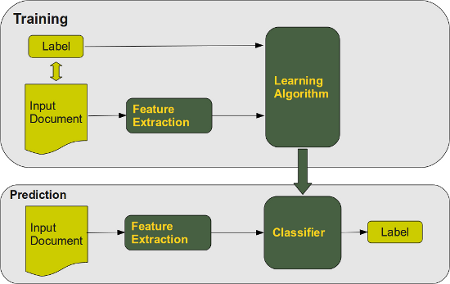
\includegraphics[height=4cm]{supervised_learning.png}
\end{center}

\end{frame}

\begin{frame}[fragile]
 \frametitle{Na\"{\i}ve Bayes Classification}
 Na\"{\i}ve Bayes is a simple probabilistic classifier based on applying Bayes' theorem or Bayes' rule. \\
 Bayes' rule $ P(H|E) = \frac{P(E|H) \times P(H)}{P(E)}$ \\
 The basic idea of Bayes's rule is that the outcome of a hypothesis or an event $(H)$ can be predicted based
on some evidences $(E)$ that can be observed.\\
 $P(H)$ is called as \emph{priori probability} . This is the probability of an event before the evidence is observed.\\
 $P(H|E)$ is called as \emph{posterior probability} . This is the probability of an event after the evidence is
observed.
\end{frame}


\begin{frame}[fragile]
 \frametitle{Na\"{\i}ve Bayes Classification}
 Let $H$ be the event of raining and $E $ be the evidence of dark cloud, then we have \\
 $ P(raining | \text{dark cloud}) = \frac{P(\text{dark cloud} | raining) \times P(raining)}{P(\text{dark cloud})} $ \\
 For multiple evidences \\
 $ P(H|E_{1},E_{2},...,E_{n}) = \frac{P(E_{1},E_{2},...,E_{n} | H) \times P(H) }{P(E_{1},E_{2},...,E_{n})}$ \\
 With the independence assumption, we can rewrite the Bayes's rule as follows: \\
 $ P(H|E_{1},E_{2},...,E_{n}) = \frac{P(E_{1}|H) \times P(E_{2}|H) \times .. P(E_{n}|H) \times P(H)}{P(E_{1},E_{2},...,E_{n})}  $
\end{frame}


\begin{frame}[fragile]
 \frametitle{Na\"{\i}ve Bayes Applied in Text Classification}
Now let's try to train a Na\"{\i}ve Bayes classifier to perform text classification. \\

$C = (terrorism,entertainment)$ \\
$D = (D_{0},D_{1},D_{2},D_{3},D_{4},D_{5})$ \\
$ BoW = (kill,bomb,kidnap,music,movie,tv) $   (vocabulary) \\
\footnotesize 
The pre-processed documents for training will look like\\
\begin{tabular}{|l|l|l|l|l|l|l|l|}
  \hline
  Training Docs & kill & bomb & kidnap & music & movie & tv & C \\ \hline
  D0 & 2 & 1 & 3 & 0 & 0 & 1 & Terrorism \\ \hline
  D1 & 1 & 1 & 1 & 0 & 0 & 0 & Terrorism \\ \hline
  D2 & 1 & 1 & 2 & 0 & 1 & 0 & Terrorism \\ \hline
  D3 & 0 & 1 & 0 & 2 & 1 & 1 & Entertainment \\ \hline
  D4 & 0 & 0 & 1 & 1 & 1 & 0 & Entertainment \\ \hline
  D5 & 0 & 0 & 0 & 2 & 2 & 2 & Entertainment \\
  \hline
  \end{tabular}
\end{frame}

\begin{frame}[fragile]
 \frametitle{Building Na\"{\i}ve Bayes Model}
Na\"{\i}ve Bayes Model for the training set will be like
\tiny[4pt]
%\fontsize{3}{1}
\begin{tabular}{|l|l|l|l|l|l|l|l|l|l|}
\hline
$|V|$&C & $P(C_{i})$ & $n_{i}$ & $P(kill|C_{i})$ & $P(bomb|C_{i})$ & $P(kidnap|C_{i})$ & $P(music|C_{i})$ & $P(movie|C_{i})$ & $P(tv|C_{i})$ \\ \hline
6 & T & 0.5 & 15 & 0.238095238 & 0.19047619 & 0.33333333 & 0.047619048 & 0.95238095 & 0.095238095 \\ \hline
 & E & 0.5 & 12 & 0.05555566 & 0.11111111 & 0.11111111 & 0.33333333 & 0.27777778 & 0.11111111 \\
\hline
\end{tabular}
\\
\normalsize
$|V|$ = the number of vocabularies = 6 \\
$P(C{i})$ = the priori probability of each class = $\frac{\text{number of documents in a class}}{\text{number of all documents}}$ \\
$n_{i}$ = the total number of word frequency in each class \\
$n_{terrorism} = 2+1+3+1+1+1+1+1+1+2+1 = 15$ \\
$n_{entertainment} = 1+2+1+1+1+1+1+2+2 = 12 $ \\
$P(w_{i} | c_{i})$ = the conditional probability of keyword occurrence given a class \\
Example \\
$P (kill | Terrorism) = \frac{(2 + 1 + 1)}{15} = \frac{4}{15}$ \\
$P (kill | Entertainment) = \frac{(0 + 0 + 0)}{ 12} = \frac{0}{12}$
\end{frame}

\begin{frame}[fragile]
 \frametitle{Building Na\"{\i}ve Bayes Model}
To avoid the “zero frequency” problem, we apply Laplace estimation by assuming a uniform distribution over all words as follows: \\
$P (kill | Terrorism) = \frac{(2 + 1 + 1 + 1)}{(15 + |V|)} = \frac{5}{21} = 0.2380 $ \\
$P (kill | Entertainment) = \frac{(0 + 0 + 0 + 1)}{(12 + |V|)} = \frac{1}{18} = 0.0555 $ \\
\end{frame}

\begin{frame}[fragile]
 \frametitle{Testing the NB model}
Our test document is \\
\begin{tabular}{|l|l|l|l|l|l|l|l|}
  \hline
  Test Docs & kill & bomb & kidnap & music & movie & tv & C \\ \hline
  Dt & 2 & 1 & 2 & 0 & 0 & 1 & ? \\ \hline
 \end{tabular} \\
To find the posterior probability :\\
\begin{displaymath}
 P(c_{i}|W) = P(c_{i}) \times \prod_{j=1}^{V} P(w_{j}|c_{i})
\end{displaymath}

\end{frame}

\begin{frame}[fragile]
 \frametitle{Testing the NB model ..}
 \tiny
 $P(Terrorism | W) = P(Terrorism) \times P(kill | Terrorism) \times P(bomb | Terrorism) \times P(kidnap | Terrorism) \times P(music | Terrorism) x P(movie | Terrorism) \times P(tv | Terrorism)$ \\
 $ = 0.5 \times 0.2380^{2} \times 0.1904^{1} \times 0.3333^{2} \times 0.0476^{0} \times 0.0952^{0} \times 0.0952^{1} $ \\
 $ = 0.5 \times 0.0566 \times 0.1904 \times 0.1110 \times 1 \times 1 \times 0.0952 $ \\
 $ = 5.7 \times 10^{-5}$ \\
 $ P(Entertainment | W) = P(Entertainment) \times P(kill | Entertainment) \times P(bomb | Entertainment) \times P(kidnap | Entertainment) \times P(music | Entertainment) \times P(movie | Entertainment) \times P(TV | Terrorism) $ \\
 $ = 0.5 \times 0.0555^{2} \times 0.1111^{1} \times 0.1111^{2} \times 0.3333^{0} \times 0.2777^{0} \times 0.1111^{1} $ \\
 $ =0.5 \times 0.0030 \times 0.1111 \times 0.0123 \times 1 \times 1 \times 0.1111 $ \\
 $ = 2.27 \times 10^{-7} $ \\
 The document has classified as "Terrorism" because it got the highest value.

\end{frame}


\begin{frame}[fragile]
 \frametitle{Preventing Underflow}
 \small
 The probability score assigned to the test document is very small. In real world situations we will train the classifier with thousands of documents. In such cases the conditional probability values will be too low for the CPU to handle. This problem is called as \emph{Underflow}. T resolve the problem we can take logarithm on the probabilities like: \\
 \tiny
 $P(Terrorism | W) = log(0.5 \times 0.2380^{2} \times 0.1904^{1} \times 0.3333^{2} \times 0.0476^{0} \times 0.0952^{0} \times 0.0952^{1})$ \\
 $ = log(0.5) + 2 log(0.2380) + 1 log(0.1904) + 2 log(0.3333) + 0 log(0.0476) + 0 log(0.0952) + 1 log(0.0952) $ \\
 $ = – 0.3010 – 1.2468 – 0.7203 – 0.9543 + 0 + 0 – 1.0213 $ \\
 $ = – 4.2437 $ \\
 $ P( Entertainment | W) = log(0.5 \times 0.0555^{2} \times 0.1111^{1} \times 0.1111^{2} \times 0.3333^{0} \times 0.2777^{0} \times 0.1111^{1}) $ \\
 $ = log(0.5) + 2 log(0.0555) + 1 log(0.1111) + 2 log(0.1111) + 0 log(0.3333) + 0 log(0.2777) + 1 log(0.1111) $ \\
 $ = = – 0.3010 – 2.511 – 0.9542 – 1.9085 + 0 + 0 – 0.9542 $ \\
 $= – 6.6289$ \\
 \small
 After handling the underflow problem our system classified the test document as "Terrorism". From the final probability score you can observe that the scores are scaled nicely. 
 \begin{block}{}
  The section on Na\"{\i}ve Bayes Classifier is prepared from the notes "A Tutorial on Naive Bayes Classification" by "Choochart Haruechaiyasak". \url{suanpalm3.kmutnb.ac.th/teacher/filedl/choochart82255418560.pdf}
 \end{block}

\end{frame}


\begin{frame}[fragile]
 \frametitle{Na\"{\i}ve Bayes Classifier }
%\footnotesize
There are two different ways to setup a Na\"{\i}ve Bayes Classifier.
\begin{itemize}
 \item Multi-variate Bernoulli Model
 \item Multinomial Model
\end{itemize}

\end{frame}

\begin{frame}[fragile]
 \frametitle{Multi-variate Bernoulli Model}
\begin{block}{Multi-variate Bernoulli Model}
 Given a vocabulary $V$, each dimension of the space $t,t \in {1,...,|V|}$ corresponds to word $w_{t}$ from the vocabulary.Dimension $t$ of the vector for document $d_{i}$ is written $B_{it}$, and is either 0 or 1, indicating whether word $w_{t}$ occurs at least once in the document. With such a document representation, we make the naive Bayes assumption: that the probability of each word occurring in a document is independent of the occurrence of other words in a document.\footnote{A Comparison of Event Models for Naive Bayes Text Classification, Andrew McCallum and Kamal Nigam, \url{http://www.cs.cmu.edu/~knigam/papers/multinomial-aaaiws98.pdf}}
\end{block}

\end{frame}

\begin{frame}[fragile]
 \frametitle{Multi-variate Bernoulli Model}
\begin{block}{Multi-variate Bernoulli Model}
 If we are adopting Multi-variate Bernoulli Model for text classification our document space representation will be like:
\footnotesize
\begin{tabular}{|l|l|l|l|l|l|l|l|}
  \hline
  Training Docs & kill & bomb & kidnap & music & movie & tv & C \\ \hline
  D0 & 1 & 1 & 1 & 0 & 0 & 1 & Terrorism \\ \hline
  D1 & 1 & 1 & 1 & 0 & 0 & 0 & Terrorism \\ \hline
  D2 & 1 & 1 & 1 & 0 & 1 & 0 & Terrorism \\ \hline
  D3 & 0 & 1 & 0 & 1 & 1 & 1 & Entertainment \\ \hline
  D4 & 0 & 0 & 1 & 1 & 1 & 0 & Entertainment \\ \hline
  D5 & 0 & 0 & 0 & 1 & 1 & 1 & Entertainment \\
  \hline
  \end{tabular} \\
\small
Here you can note that the individual word frequency has been replaced by presence or absence of the word.
\end{block}

\end{frame}

\begin{frame}[fragile]
 \frametitle{Multinomial Model}
\footnotesize
\begin{block}{Multinomial Model}
 In contrast to the multi-variate Bernoulli event model, the multinomial model captures word frequency information in documents.In the multinomial model, a document is an ordered sequence of word events, drawn from the same vocabulary $V$. We again make a similar naive Bayes assumption: that the probability of each word event in a document is independent of the word's context and position in the document.
\end{block}
\scriptsize
In the NB example which we worked out we applied the multinomial model. In the model we used simple bag of words representation. We an use smoothed bag of words mode like TF-IDF in the multinomial naive bayes model. 
\end{frame}


\begin{frame}
 \frametitle{Support Vector Machine}
 Support Vector Machine is an abstract learning machine; which learns from a training set attempts to generalize and makes correct predictions on new data. Consider a training set : $ \{(x_{i},y_{i})\}^{n} _{i=1}$  where  $x_{i} \in \mathbb{R}^{p}$ (input feature vector) and $y_{i} \in \{1,-1\}$ is corresponding label whether $(y_{i} = +1)$ or $(y_{i} = -1)$ . To start with we assume that our input feature vectors are linearly separable, that is there exists a function $f(x) = \langle w,x \rangle + b $ where $w \in \mathbb{R}^{p}$ (weight vector) and $b \in \mathbb{R}$ (bias) such that \\
 \vspace{0.3 cm}
 $\langle w, x_{i} \rangle + b > 0 $ for $y_{i} = +1 $ \\
 $\langle w,x_{i} \rangle + b < 0 $ for $y_{i} = -1 $ \\
 \vspace{0.3 cm}
 $\langle w, x \rangle + b = 0 $ is the decision hyperplane. There can be multiple hyperplanes which can separate positive and negative examples.  But all of them are not equal. SVM tries to find the particular hyperplane that maximizes the margin. The vectors which is closer to the maximum margin is calles as support vectors. If the data is not linearly separable we have to use Kernel tricks to find soft margins. 
\end{frame}


\begin{frame}[fragile]
 \frametitle{Support Vector Machine}
\footnotesize
\justifying 
Suppose a bunch of red square and blue rectangle figures are scattered over a table. If the figures are mixed then it is not possible to separate in a \emph{linear} way. \\
If there is a clear blank space available in the table in between the square and rectangles; we can say that it is \emph{linearly separable}. A line which drawn in the clear space between the figures,exactly equal length from the margin of scatter region of square and rectangle is called as \emph{separating hyperplane}. Everything on the one side of the separating hyper plane belongs to one category, and everything in the other side belongs to the other category (red square and blue rectangles). A line drawn in the edges of each scatter (square and rectangle) in an equal distance from the \emph{separating hyperplane} is called \emph{maximum margin}. The figures closest to the separating hyperplane are known as \emph{support vectors}.\footnote{This is just a non theoretic definition "just to get an idea only". For more refer \url{http://www.statsoft.com/textbook/support-vector-machines/} and bibiliography} If the data is not \emph{linearly separable} we have to use kernel tricks \footnote{\url{http://www.
statsoft.com/textbook/support-vector-machines/}}.
\end{frame}

\begin{frame}
 \frametitle{Support Vector Machine}
 \begin{center}
  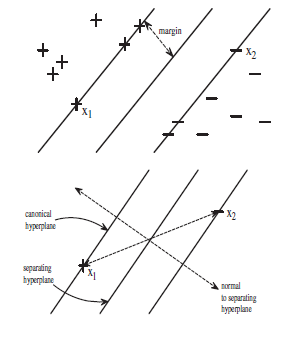
\includegraphics[height=7cm]{svm.png}
 \end{center}

\end{frame}


\begin{frame}[fragile]
 \frametitle{Practice Time}
\footnotesize
Let's try to build a Multinomial Na\"{\i}ve Bayes Classifier with Python Sklearn.
\tiny
\begin{verbatim}
from sklearn.datasets import load_files
from sklearn.feature_extraction.text import CountVectorizer
from sklearn.feature_extraction.text import TfidfTransformer

from sklearn.pipeline import Pipeline
from sklearn.naive_bayes import MultinomialNB

dir_data = "/usr/share/nltk_data/corpora/movie_reviews/" #replace with your path

vectorizer = CountVectorizer(analyzer = 'word',ngram_range = (1,3),\
    stop_words='english',lowercase=True)
transformer = TfidfTransformer(use_idf=True)
classifier = Pipeline([('vect',vectorizer),('tfidf',transformer),\
    ('clf',MultinomialNB()),])

categories = ['pos','neg']
training_data = load_files(dir_data,categories=categories,\
    shuffle = True)

 _ = classifier.fit(training_data.data, training_data.target)

print training_data.target_names[classifier.predict(['This is a good one'])]
\end{verbatim}

\end{frame}


\begin{frame}[fragile]
 \frametitle{Practice Time}
\footnotesize
Let's try to build a SVM Classifier with Python Sklearn.
\tiny
\begin{verbatim}
from sklearn.datasets import load_files
from sklearn.feature_extraction.text import CountVectorizer
from sklearn.feature_extraction.text import TfidfTransformer

from sklearn.pipeline import Pipeline
from sklearn.svm import LinearSVC

dir_data = "/usr/share/nltk_data/corpora/movie_reviews/" #replace with your path

vectorizer = CountVectorizer(analyzer = 'word',ngram_range = (1,3),\
    stop_words='english',lowercase=True)
transformer = TfidfTransformer(use_idf=True)
classifier = Pipeline([('vect',vectorizer),('tfidf',transformer),\
    ('clf',LinearSVC()),])

categories = ['pos','neg']
training_data = load_files(dir_data,categories=categories,\
    shuffle = True)

 _ = classifier.fit(training_data.data, training_data.target)

print training_data.target_names[classifier.predict(['This is a good one'])]
\end{verbatim}

\end{frame}

\begin{frame}[fragile]
 \frametitle{Practice Time}
\footnotesize
Let's try to build a Multi-variate Na\"{\i}ve Bayes Classifier with Python NLTK \footnote{This code is adopted from \url{http://streamhacker.com/2010/05/10/text-classification-sentiment-analysis-naive-bayes-classifier/}. Follow the link for more detailed discussion}.
\tiny
\begin{verbatim}
import nltk.classify.util
from nltk.classify import NaiveBayesClassifier
from nltk.corpus import movie_reviews

def word_feats(words):
    return dict([(word, True) for word in words])

negids = movie_reviews.fileids('neg')
posids = movie_reviews.fileids('pos')

negfeats = [(word_feats(movie_reviews.words(fileids=[f])), \
        'neg') for f in negids]
posfeats = [(word_feats(movie_reviews.words(fileids=[f])), \
        'pos') for f in posids]

negcutoff = len(negfeats)*3/4
poscutoff = len(posfeats)*3/4

trainfeats = negfeats[:negcutoff] + posfeats[:poscutoff]

classifier = NaiveBayesClassifier.train(trainfeats)

sent = "This is really cool. I like it"
words = word_feats(sent.lower().split())

print classifier.classify(words)
\end{verbatim}

\end{frame}

\begin{frame}[fragile]
 \frametitle{Evaluating Performance of a Classifier}
\begin{block}{Confusion Matrix}
 Confusion matrix is a specific table layout that allows visualization of the performance of an algorithm.
\end{block}
\vspace{.5cm}
Consider that we built a classifier with two categories "Positive" and "Negative". A confusion matrix for the classifier will look like: \\
\vspace{.5cm}
\footnotesize
\begin{tabular}{|l|l|c|c|c}
 \cline{3-4}
 \multicolumn{2}{c|}{}& \multicolumn{2}{c|}{Actual}&\\
 \cline{3-4}
 \multicolumn{2}{c|}{}&Positive&Negative&\\
 \cline{1-4}
 \multirow{2}{*}{Predicted}& Positive & \cellcolor{orange!25} True Positive (TP) & False Positive (FP) & \\
 \cline{2-4}
 & Negative & False Negative (FN) & \cellcolor{orange!25} True Negative (TN) & \\
 \cline{1-4}
 \end{tabular}
\end{frame}

\begin{frame}
  \frametitle{Evaluating Performance of a Classifier}
\begin{block}{Accuracy of a Classifier}
\begin{center}
  $Accuracy = \frac{TP + TN}{TP + FP + FN + TN} $
\end{center}
\end{block}
\vspace{.5cm}
\footnotesize
\begin{tabular}{|l|l|c|c|c|}
 \cline{3-5}
 \multicolumn{2}{c|}{}& \multicolumn{2}{c}{Actual}&\\
 \cline{3-5}
 \multicolumn{2}{c|}{}&Positive&Negative&Total\\
 \cline{1-5}
 \multirow{2}{*}{Predicted}& Positive & \cellcolor{orange!25}  562 & 77 & 639\\
 \cline{2-5}
 & Negative & 225 & \cellcolor{orange!25} 436 & 661\\
 \cline{2-5}
 & Total & 787 & 513 & 1300\\
\cline{1-5}
 \end{tabular} \\
\vspace{.5cm}
\footnotesize
Accuracy = $ \frac{562 + 436}{ 562 + 77 + 225 + 436} = 0.76$
\end{frame}

\begin{frame}
 \frametitle{Evaluating Performance of a Classifier}
 \begin{block}{Precision and Recall}
Precision, which indicates how many of the items that we identified were relevant\\
\vspace{.5cm}
  $Precision = \frac{TP}{TP + FP}$ \\
\vspace{.5cm}
Recall, which indicates how many of the relevant items that we identified. It is equivalent with "hit rate" and "sensitivity". \\
\vspace{.5cm}
$Recall = \frac{TP}{TP + FN}$
 \end{block}

\end{frame}

\begin{frame}
 \frametitle{Evaluating Performance of a Classifier}
\begin{tabular}{|l|l|c|c|c|}
 \cline{3-5}
 \multicolumn{2}{c|}{}& \multicolumn{2}{c}{Actual}&\\
 \cline{3-5}
 \multicolumn{2}{c|}{}&Positive&Negative&Total\\
 \cline{1-5}
 \multirow{2}{*}{Predicted}& Positive & \cellcolor{orange!25}  562 & 77 & 639\\
 \cline{2-5}
 & Negative & 225 & \cellcolor{orange!25} 436 & 661\\
 \cline{2-5}
 & Total & 787 & 513 & 1300\\
\cline{1-5}
 \end{tabular} \\
\vspace{.5cm}
\footnotesize
Positive Precision = $ \frac{562 }{ 562 + 77 } = 0.87$ \\
Negative Precision = $ \frac{436 }{ 225 + 436 } = 0.65$ \\
Positive Recall = $ \frac{562 }{ 562 + 225 } = 0.71$ \\
Negative Recall = $ \frac{436 }{ 77 + 436 } = 0.84$ 
\end{frame}


\begin{frame}
 \frametitle{Evaluating Performance of a Classifier}
\begin{block}{Error Rate}
 Error rate is the percentage of things done wrong.\\
\vspace{.5cm}
 $Error Rate = \frac{FP+FN}{TP+FP+FN+TN}$
\end{block}
\vspace{.5cm}
\begin{tabular}{|l|l|c|c|c|}
 \cline{3-5}
 \multicolumn{2}{c|}{}& \multicolumn{2}{c}{Actual}&\\
 \cline{3-5}
 \multicolumn{2}{c|}{}&Positive&Negative&Total\\
 \cline{1-5}
 \multirow{2}{*}{Predicted}& Positive & \cellcolor{orange!25}  562 & 77 & 639\\
 \cline{2-5}
 & Negative & 225 & \cellcolor{orange!25} 436 & 661\\
 \cline{2-5}
 & Total & 787 & 513 & 1300\\
\cline{1-5}
 \end{tabular} \\
\vspace{.5cm}
$Error Rate = \frac{77+225}{562+77+225+436} = 0.23$
\end{frame}
%FP / (FP+TN)
\begin{frame}
 \frametitle{Evaluating Performance of a Classifier}
\begin{block}{Fall-out}
 It is a proportion of non relevant item that were mistakenly selected. It is equivalent with false positive rate (FPR).\\
 \vspace{.5cm}
 $ Fall-out = \frac{FP}{FP + TN}$
\end{block}
\vspace{.5cm}
\begin{tabular}{|l|l|c|c|c|}
 \cline{3-5}
 \multicolumn{2}{c|}{}& \multicolumn{2}{c}{Actual}&\\
 \cline{3-5}
 \multicolumn{2}{c|}{}&Positive&Negative&Total\\
 \cline{1-5}
 \multirow{2}{*}{Predicted}& Positive & \cellcolor{orange!25}  562 & 77 & 639\\
 \cline{2-5}
 & Negative & 225 & \cellcolor{orange!25} 436 & 661\\
 \cline{2-5}
 & Total & 787 & 513 & 1300\\
\cline{1-5}
 \end{tabular} \\
\vspace{.5cm}
$Fall-out = \frac{77}{77+436} = 0.15$
%$Fall-out = \frac{225}{225+502} = 0.30$
\end{frame}

\begin{frame}
\frametitle{Evaluating Performance of a Classifier}
 \begin{block}{F1 Score}
  In statistics, the F1 score (also F-score or F-measure) is a measure of a test's accuracy. It considers both the precision p and the recall r of the test to compute the score: p is the number of correct results divided by the number of all returned results and r is the number of correct results divided by the number of results that should have been returned. The F1 score can be interpreted as a weighted average of the precision and recall, where an F1 score reaches its best value at 1 and worst score at 0 \footnote{\url{http://en.wikipedia.org/wiki/F1\_score}}.\\
\vspace{.5cm}
F1 Score $ = 2 . \frac{precision . recall}{precision + recall}$
 \end{block}

\end{frame}

\begin{frame}
 \frametitle{Evaluating Performance of a Classifier}
F1 Score Positive  $= 2 . \frac{0.87 . 0.71}{0.87 + 0.71} = 0.78$ \\
F1 Score Positive $= 2 . \frac{0.65 . 0.84}{0.65 + 0.84} = 0.73$
\end{frame}

\begin{frame}
\frametitle{Evaluating Performance of a Classifier}
 \begin{block}{Positive predictive value}
  Positive predictive value, or precision rate is the proportion of positive test results that are true positives.\\
\vspace{.5cm}
 Positive predictive value $= \frac{TP}{TP+FP} $
 \end{block}
\vspace{.5cm}
Positive predictive value $= \frac{562}{562+77} = 0.87$
\end{frame}

\begin{frame}
\frametitle{Evaluating Performance of a Classifier}
 \begin{block}{Negative predictive value}
  Negative predictive value (NPV) is a summary statistic used to describe the performance of a diagnostic testing procedure.\\
\vspace{.5cm}
$NPV = \frac{TN}{TN+FN}$
 \end{block}
\vspace{.5cm}
$NPV = \frac{436}{436+225} = 0.65$
\end{frame}

\begin{frame}
 \frametitle{Evaluating Performance of a Classifier}
 \begin{block}{Specificity or True Negative Rate}
  Specificity $= \frac{TN}{FP + TN}$
 \end{block}
 \vspace{.5cm}
 Specificity = $ = \frac{436}{77 + 436} = 0.84$

\end{frame}

\begin{frame}
 \frametitle{Evaluating Performance of a Classifier}
 \begin{block}{False Discovery Rate}
  False discovery rate (FDR) control is a statistical method used in multiple hypothesis testing to correct for multiple comparisons.\\
  \vspace{.5cm}
  $FDR = \frac{FP}{FP+TP}$
 \end{block}
\vspace{.5cm}
$FDR = \frac{77}{77+562} = 0.12$
\end{frame}


\begin{frame}
 \frametitle{Evaluating Performance of a Classifier}
\begin{block}{Matthews Correlation Coefficient}
The Matthews Correlation Coefficient (MCC) is used in machine learning as a measure of the quality of binary (two-class) classifications.\\
\vspace{.5cm}
$MCC = \frac{TP \times TN - FP \times FN}{\sqrt {(TP+FP) (TP+FN) (TN+FP) (TN+FN)}}$
\end{block}
\vspace{.5cm}
$MCC =\frac{562 \times 436 - 77 \times 225}{\sqrt{(562+77)(562+225)(436+77)(436+225)}} = 0.55$
%http://en.wikipedia.org/wiki/Matthews_correlation_coefficient
\end{frame}

\begin{frame}
 \frametitle{Evaluating Performance of a Classifier}
%http://docs.oracle.com/cd/E11882_01/datamine.112/e16808/classify.htm
\begin{block}{Receiver Operating Characteristic (ROC)}
 ROC is another metric for comparing predicted and actual target values in a classification model. It applies to the binary classification problem.ROC can be plotted as a curve on an X-Y axis. The false positive rate is placed on the X axis. The true positive rate is placed on the Y axis.The top left corner is the optimal location on an ROC graph, indicating a high true positive rate and a low false positive rate.
\end{block}

\end{frame}

\begin{frame}
 \frametitle{Evaluating Performance of a Classifier}
\begin{block}{Area Under the Curve}
 The area under the ROC curve (AUC) measures the discriminating ability of a binary classification model. The larger the AUC, the higher the likelihood that an actual positive case will be assigned a higher probability of being positive than an actual negative case. The AUC measure is especially useful for data sets with unbalanced target distribution (one target class dominates the other).
\end{block}

\end{frame}


\begin{frame}
 \frametitle{Named Entity Recognition}
\begin{block}{Named Entity Recognition}
 Named-entity recognition (NER) (also known as entity identification and entity extraction) is a sub-task of information extraction that seeks to locate and classify atomic elements in text into predefined categories such as the names of persons, organizations, locations, expressions of times, quantities, monetary values, percentages, etc.
\end{block}

\end{frame}

\begin{frame}[fragile]
 \frametitle{Named Entity Recognition}
\footnotesize
Entity Recognition with Python NLTK
\begin{verbatim}
from nltk import sent_tokenize, ne_chunk, pos_tag, word_tokenize

def extract_entities(text):
    entities = []
    sents = sent_tokenize(text)
    chunks = [ ne_chunk(pos_tag(word_tokenize(sent)),\
    binary=True) for sent in sents]
    for chunk in chunks:
        for tree in chunk.subtrees():
            if tree.node == "NE":
                entity = ' '.join(leaf[0] for leaf in tree.leaves())
                entities.append(entity)
    return entities

if __name__ == "__main__":
    sent = "Abraham Lincoln was born February 12, 1809, the second child \
    of Thomas Lincoln and Nancy Lincoln."
    entities = extract_entities(sent)
    print entities

\end{verbatim}

\end{frame}

\begin{frame}[fragile]
 \frametitle{Extracting Terms from Text}
Extracting Terms with Python Topia Termextract \footnote{\url{http://pypi.python.org/pypi/topia.termextract/}} \\
\begin{verbatim}
from topia.termextract import extract

extractor = extract.TermExtractor()

text = "Abraham Lincoln was born February 12, 1809, the \
second child of Thomas Lincoln and Nancy Lincoln."

terms = extractor(text)
terms = [term[0] for term in terms]

print terms

\end{verbatim}

\end{frame}


%%%%%%%%%%%%%%%%%%%%%%%%%%%%%%%
%Ref
\begin{frame}
 \frametitle{References}
\footnotesize
\begin{thebibliography}{9}
 \bibitem{1} Chris Smith,Machine Learning: Text Feature Extraction (tf-idf) - Part I,\url{ http://css.dzone.com/articles/machine-learning-text-feature}, Accessed on 20th Sept. 2012. 
 \bibitem{2} Chris Smith, Machine Learning: Text Feature Extraction (tf-idf) - Part II, \url{http://css.dzone.com/articles/machine-learning-text-feature-0?mz=55985-python}, Accessed on 20th Sept. 2012.
 \bibitem{3} Pierre M. Nugues, An Introduction to Language Processing with Perl and Prolog, Springer,2006.
 \bibitem{4} Kenneth W. Church and Robert L. Mercer,Introduction to the Special Issue on Computational Linguistics Using Large Corpora,  \url{acl.ldc.upenn.edu/J/J93/J93-1001.pdf}, Accessed on 23rd Sept 2012.
\bibitem{5} Roger Bilisoly,Practical Text Mining with Perl, Wiley, 2008.
\bibitem{6} , Text Categorization and Classification, \url{http://www.python-course.eu/text_classification_introduction.php}
\end{thebibliography}
\end{frame}

\begin{frame}
 \frametitle{References}
\footnotesize
\begin{thebibliography}{9}
 \bibitem{7} Chris Manning and Hinrich Schütze, Foundations of Statistical Natural Language Processing, MIT Press. Cambridge, MA: May 1999.
 \bibitem{8} Choochart Haruechaiyasak, A Tutorial on Naive Bayes Classification, \url{suanpalm3.kmutnb.ac.th/teacher/filedl/choochart82255418560.pdf}, Accessed on Feb 10 2012. 
 \bibitem{9} Andrew McCallum and Kamal Nigam, A Comparison of Event Models for Naive Bayes Text Classification, \url{http://www.cs.cmu.edu/~knigam/papers/multinomial-aaaiws98.pdf}, Accessed on March 2, 2012. 
 \bibitem{10} Jimmy Lin,Scalable Language Processing Algorithms for the Masses: A Case Study in Computing Word Co-occurrence Matrices with MapReduce, \url{www.aclweb.org/anthology/D08-1044}
 \bibitem{11} Christopher D. Manning, Prabhakar Raghavan and Hinrich Schütze, Introduction to Information Retrieval, Cambridge University Press. 2008.
\end{thebibliography}

\end{frame}

%%%%%%%%%%%%%%%%%%%%%%%%%%%%%%$$
\end{document}
